\documentclass{scrbook}
\usepackage[ngerman]{babel}
\usepackage[T1]{fontenc}
\usepackage[ansinew]{inputenc}
\usepackage{a4wide}

%verwenden von grafiken
\usepackage[dvipdf, final]{graphicx}

%verwenden von hyperlinks, stil derselben
\usepackage{color}
\definecolor{darkblue}{rgb}{0,0,0.5}

\usepackage{hyperref}
\hypersetup{
%	draft,										%hyperlinks ausschalten				
	colorlinks,									%hyperlinks farbig darstellen
	linkcolor   = darkblue,
	filecolor   = darkblue,
	urlcolor    = darkblue,
	citecolor   = darkblue,
	pdftitle    = {Handbuch},	%titel
	pdfsubject  = {j-Algo},			%thema
	pdfauthor   = {Alexander Claus, Matthias Schmidt},
	pdfkeywords = {Algorithmen, Visualisierung},
	pdfcreator  = {Distiller},
	pdfproducer = {LaTeX mit Hyperref-Package}}

%spezielle kommandos
%schreibweise des software-titels
\newcommand{\jalgo}{\mbox{\bfseries j-Algo} }
%pfad zu den bildern
\newcommand{\pfad}{pics/}
%f�gt ein bild an einer bestimmten stelle, relativ zur position des befehls, ein.
%usage: \icon{dateiname}{y-offset}{x-offset}{bildvergr��erung}
\newcommand{\icon}[4]{
	\vspace{#2 ex}
	\hspace{#3 ex}
	\includegraphics[scale=#4]{\pfad #1}
}
%f�gt ein bild mittig mit bildunterschrift ein.
%usage: \centerpic{dateiname}{bildvergr��erung}{untertitel}
\newcommand{\centerpic}[3]{
	\begin{center}
		\includegraphics[scale=#2]{\pfad #1}\\
		{\small #3}
	\end{center}
}
%f�gt eine \subsection mit einem f�hrenden icon ein
%usage: \subsectionicon{text}{icon}
\newcommand{\subsectionicon}[2]{
	\subsection[#1]{\qquad #1}
	\icon{#2}{-5}{7}{1}
	\\
}
%f�gt eine \subsection mit 2 f�hrenden icons ein
%usage: \subsectiondoubleicon{text}{icon1}{icon2}
\newcommand{\subsectiondoubleicon}[3]{
	\subsection[#1]{\qquad \quad #1}
	\icon{#2}{-5}{7}{1}
	\icon{#3}{0}{-2}{1}
	\\
}
%f�gt eine \subsubsection* mit 2 f�hrenden icons ein
%usage: \subsubsectiondoubleicon{text}{icon1}{icon2}
\newcommand{\subsubsectiondoubleicon}[3]{
	\subsubsection*{\qquad \qquad #1}
	\icon{#2}{-4}{1}{1}
	\icon{#3}{0}{-2}{1}
	\\
}

\begin{document}

\begin{titlepage}
\centerpic{main/title}{1}{}
\vfill
\begin{flushright}
{\Huge \textbf{Benutzerhandbuch}}
\end{flushright}
\end{titlepage}

\newpage

\tableofcontents
\newpage

\part{Das Hauptprogramm}
\chapter{Das Modul Dijkstra}
\section{Einleitung}
Das Modul \dijkstra visualisiert den bekannten Algorithmus von E. W. Dijkstra zum Finden der k�rzesten Wege von einem Startknoten in einem Distanzgraphen. Der Algorithmus selbst ist unter anderem im Vorlesungsskript von Prof. Vogler "`Algorithmen, Datenstrukturen und Programmierung"' zu finden. Aber auch im Internet existieren zahlreiche Quellen dazu.

Soweit es m�glich gewesen ist, wurde beim Design des Moduls darauf geachtet, es weitgehend intuitiv und selbst-dokumentierend zu gestalten. Nichtsdestotrotz findet sich hier eine kurze
Einf�hrung in das \dijkstra - Modul.

\section{Funktions�bersicht}
Das Modul \dijkstra realisiert folgende Funktionen:
\begin{itemize}
	\item graphisches Erstellen / Bearbeiten eines Distanzgraphen
	\item Erstellen / Bearbeiten eines Graphen mittels Kanten- / Knotenliste oder Adjazenzmatrix
	\item Speichern und Laden von Graphen
	\item Visualisierung des Dijkstra-Algorithmus
\end{itemize}

\section{Modul starten}
Um das Modul zu starten, w�hlt man im Men� \textsc{<Datei>} das Submen� \textsc{<Neu>} und dann den Men�befehl \textsc{\dijkstra}. Im Hauptfenster erscheint nun die Oberfl�che des \dijkstra - Moduls im Eingabe-Modus.

\section{Symbolleiste}
Die Symbolleiste stellt die Funktionen \textsc{Speichern, Speichern unter, R�ckg�ngig} und \textsc{Wiederherstellen} bereit.
\newpage
\section{Grundfunktionen}
\jalgo bietet eine Reihe von Grundfunktionen, die unabh�ngig von den Modulen zur Verf�gung stehen, bzw. f�r jedes Modul die gleiche Bedeutung haben. Im Einzelnen sind das das �ffnen von Modulen sowie das Laden und Speichern von Sitzungsdaten. Die Grundfunktionen sind �ber die Werkzeugleiste oder den Men�punkt <\textsc{Datei}> erreichbar.

\subsectionicon{Neues Modul �ffnen}{main/icon_new}
Ein Klick auf den Button <\textsc{Neu}> in der Werkzeugleiste gibt Ihnen die M�glichkeit, ein beliebiges neues Modul zu �ffnen. Dabei wird ein Auswahldialog ge�ffnet, in welchem die installierten Module aufgelistet sind. Hier werden Ihnen au�erdem kurze Informationen zu diesen Modulen angezeigt. Sie k�nnen w�hlen, ob dieser Auswahldialog bei jedem Start des Programmes angezeigt werden soll oder nicht.\\
Alternativ dazu kann �ber das Men� \textsc{<Datei>$\rightarrow$<Neu>} das gew�nschte Modul geladen werden. Dies ist der schnellere Weg und zu empfehlen, wenn man bereits einen �berblick �ber die installierten Module hat.

\subsectionicon{Gespeicherte Sitzungsdaten laden}{main/icon_open}
Mit einem Klick auf den Button <\textsc{�ffnen}> erscheint ein Dialog zur Dateiauswahl. Hier haben Sie die M�glichkeit, eine Datei auszuw�hlen, in welcher modulspezifische Sitzungsdaten gespeichert wurden. Die Dateien, die von \jalgo gespeichert werden, tragen die Dateiendung \emph{"`.jalgo"'}.\\
Achtung: Da jedes Modul von \jalgo seine Daten in einer solchen Datei ablegt, kann man beim Blick auf die unge�ffnete Datei nicht erkennen, mit welchem Modul diese assoziiert wurde. Es wird jeweils das assoziierte Modul zu der geladenen Datei ge�ffnet. Achten Sie daher bei der Vergabe der Dateinamen auf m�glichst eindeutige Bezeichner.\\
Anmerkung: In einer sp�teren Version wird direkt bei der Dateiauswahl das zugeh�rige Modul mit angezeigt.
\centerpic{main/loaddialog}{0.45}{Das Dialogfenster zum �ffnen}

\medskip
\subsectiondoubleicon{Sitzungsdaten speichern}{main/icon_save}{main/icon_save_as}
Per Klick auf die Buttons <\textsc{Speichern}> und <\textsc{Speichern unter}> k�nnen Sie die Sitzungsdaten des gerade aktiven Moduls in einer Datei speichern. Wie beim Laden �ffnet sich auch hier ein Dialog zur Dateiauswahl, in welchem Sie Zielpfad und Name der neuen Datei eintragen k�nnen. Die Angabe der Dateiendung ist nicht n�tig, das Programm 
erg�nzt diese automatisch.\\
Je nach Implementierung des aktiven Moduls steht die Speicherfunktion nur zur Verf�gung, wenn gerade kein Algorithmus l�uft. Sollte noch ein Algorithmus aktiv sein, so beenden Sie diesen bitte vorher oder brechen ihn ab.

\subsection{Modul schlie�en}
Sie haben die M�glichkeit, jede Modulinstanz durch Klick auf das Kreuz der dazugeh�rigen Registerkarte zu schlie�en. Dabei werden Sie gegebenenfalls gefragt, ob Sie Ihre Arbeit speichern wollen. Um das gesamte Programm zu schlie�en, ist es nicht n�tig, die Module einzeln zu schliessen, das erledigt das Programm f�r Sie.

\bigskip
\begin{center}
	\raisebox{-7ex}{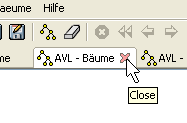
\includegraphics[scale=0.8]{\pfad main/closebutton}} \hfill
	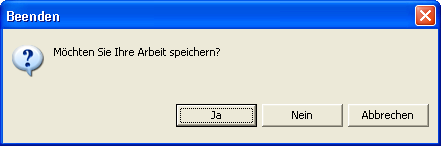
\includegraphics[scale=0.55]{\pfad main/closemessage} \\
	{\small Der Knopf zum Schlie�en eines Moduls.} \hfill
	{\small Die Abfrage, ob die Daten gespeichert werden sollen.}
\end{center}

\subsectionicon{Hilfe}{main/icon_help}
Die Hilfe stellt ein wichtiges Nachschlagewerk f�r all diejenigen dar, die nicht auf Anhieb mit allen Funktionen von \jalgo und seinen Modulen klar kommen. Hier k�nnen Sie noch einmal eine genaue Beschreibung zu den einzelnen Programmelementen nachlesen.\\
Die Hilfe ist kontextspezifisch aufgebaut, d.h. ist ein Modul ge�ffnet, so wird in der Hilfe automatisch an die entsprechende Stelle gesprungen.\\
Sie erreichen die Hilfe �ber den Men�punkt \textsc{<Hilfe>$\rightarrow$<Inhalt>} oder indem Sie einfach auf die Taste <\textsc{F1}> Ihrer Tastatur dr�cken.

\subsection{Hinweis-Tipps}
Zus�tzlich wird zu den meisten Kontrollelementen, also Buttons, Men�eintr�ge, etc., ein kurzer Hinweistext neben dem Mauszeiger bzw. in der Statuszeile des Programmes angezeigt. Dies sollte als schnelle Hilfestellung den meisten Anforderungen gen�gen.

\newpage
\section{Impressum}
Das Modul KMP wurde im Sommersemester 2006 von der Praktikumsgruppe SWT06-13 im Rahmen des externen Softwarepraktikums entwickelt. Mitwirkende waren die
\paragraph{Teammitglieder}
\begin{itemize}
	\item Danilo Lisske --- Chefprogrammierer
	\item Sebastian Patschorke  --- Assistent
	\item Matthias Neubert --- Testverantwortlicher
	\item 	Elisa B�hl --- Sekret�r
	\item Nadine Grabow --- Administrator
\end{itemize}
sowie der betreuende Tutor Matthias Schmidt.\\
Die Webseite des Projektes finden Sie unter \href{http://web.inf.tu-dresden.de/~swt06-13/}{http://web.inf.tu-dresden.de/\~{}swt06-13/}.

Das Handbuch zu diesem Modul wurde erstellt von Nadine Grabow.

\part{Die Module}
\newcommand{\ebnf}{\mbox{\bfseries EBNF und Syntaxdiagramme} }

\chapter{Das Modul Dijkstra}
\section{Einleitung}
Das Modul \dijkstra visualisiert den bekannten Algorithmus von E. W. Dijkstra zum Finden der k�rzesten Wege von einem Startknoten in einem Distanzgraphen. Der Algorithmus selbst ist unter anderem im Vorlesungsskript von Prof. Vogler "`Algorithmen, Datenstrukturen und Programmierung"' zu finden. Aber auch im Internet existieren zahlreiche Quellen dazu.

Soweit es m�glich gewesen ist, wurde beim Design des Moduls darauf geachtet, es weitgehend intuitiv und selbst-dokumentierend zu gestalten. Nichtsdestotrotz findet sich hier eine kurze
Einf�hrung in das \dijkstra - Modul.

\section{Funktions�bersicht}
Das Modul \dijkstra realisiert folgende Funktionen:
\begin{itemize}
	\item graphisches Erstellen / Bearbeiten eines Distanzgraphen
	\item Erstellen / Bearbeiten eines Graphen mittels Kanten- / Knotenliste oder Adjazenzmatrix
	\item Speichern und Laden von Graphen
	\item Visualisierung des Dijkstra-Algorithmus
\end{itemize}

\section{Modul starten}
Um das Modul zu starten, w�hlt man im Men� \textsc{<Datei>} das Submen� \textsc{<Neu>} und dann den Men�befehl \textsc{\dijkstra}. Im Hauptfenster erscheint nun die Oberfl�che des \dijkstra - Moduls im Eingabe-Modus.

\section{Symbolleiste}
Die Symbolleiste stellt die Funktionen \textsc{Speichern, Speichern unter, R�ckg�ngig} und \textsc{Wiederherstellen} bereit.
\newpage
\section{Der Willkommensbildschirm}
\label{sec:DerWillkommensbildschirm}

\subsection{Modul KMP starten}
\label{sec:ModulKMPStarten}

Nach Starten des Hauptprogramms j-Algo k�nnen Sie �ber den Button 'Neu' oder mit dem Men�punkt 'Datei' => 'Neu' eine neue Instanz des Moduls KMP �ffnen. Anschlie�end �ffnet sich der Willkommensbildschirm des Moduls, der Ihnen verschiedene M�glichkeiten er�ffnet.			
		
\bigskip
\centerpic{kmp/welcomescreen}{0.5}{Der Willkommensbildschirm des Moduls}
\bigskip

\subsectionicon{Generierung der Verschiebetabelle}{kmp/welcome_phaseone}
Mit Klick auf das erste Symbol gelangen Sie zur ersten Phase des KMP-Algorithmus, in dem f�r ein Pattern die Verschiebetabelle erstellt wird.

\subsectionicon{ Suchen im Suchtext}{kmp/welcome_phasetwo} 
Mit Klick auf das zweite Symbol gelangen Sie zur zweiten Phase des KMP-Algorithmus, in dem ein Text nach einem Pattern durchsucht wird.

\subsectionicon{ �ffnen einer KMP-Sitzung}{kmp/welcome_open}  
Mit Klick auf das Ordner-Symbol erhalten Sie die M�glichkeit, ein zuvor gespeichertes KMP-Beispiel zu laden ("*.jalgo" - Datei)

\subsectionicon{ Pr�sentation von Lernbeispielen}{kmp/welcome_example}   
Mit Klick auf das Tafel-Symbol erhalten Sie die M�glichkeit, anhand gegebener repr�sentativer Lernbeispiele die Funktions- und Arbeitsweise des Algorithmus kennenzulernen.
\section{EBNF-Definitionen}

\subsection{Der EBNF-Editor}

\subsubsection{Die Arbeitsfl�che}

Die Arbeitsfl�che der EBNF-Eingabe teilt sich in eine obere und eine untere H�lfte. Die obere H�lfte dient der Eingabe der Definition, die untere der Ansicht. \\

Ein nachtr�gliches Bearbeiten der Definition wird durch die Interaktivit�t der Definition im unteren Bereich erm�glicht.

\centerpic{ebnf/ebnfinput_full.png}{.7}{Die Arbeitsfl�che des Moduls \ebnf}
\bigskip

\subsubsection{Eingabe einer Definition}

Die Definition wird im oberen Bilschirmbereich eingegeben. Es stehen Steuerelemente f�r die Eingabe von Variablen, Terminalsymbolen sowie Regeln zur Verf�gung.

\begin{itemize}
	\item Eingabe von Variablen und Terminalsymbolen

	\begin{itemize}
		\item Zugelassene Symbole \\
					Grunds�tzlich sind alle Symbole zugelassen, die die folgenden Bedingungen 	
					erf�llen:

		\begin{itemize}
			\item Ein Symbol darf nicht der Anfang eines anderen Terminalsymbols oder 
					  einer anderen Variable sein
      \item Ein Symbol darf nicht mit Leerzeichen beginnen oder enden
      \item Ein Symbol darf nicht leer sein
      \item Ein Symbol darf keine Metasymbole enthalten 
		\end{itemize}
		
    \item Hinzuf�gen von Terminalsymbolen und Variablen zur EBNF-Definition \\
    			Das hinzuzuf�gende Symbol muss in das entsprechende Textfeld geschrieben werden
    			und kann dann mit der Eingabetaste oder Klick auf Hinzuf�gen zur Definition
    			hinzugef�gt werden. Falls das Symbol nicht hinzugef�gt werden kann, wird eine
    			entsprechende Fehlermeldung angezeigt.
    			
    			\begin{center}
						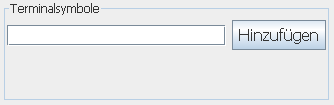
\includegraphics[scale=0.5]{\pfad ebnf/ebnfinput_addterminal.png} \hfill
						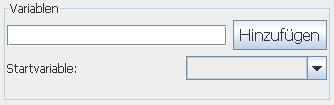
\includegraphics[scale=0.5]{\pfad ebnf/ebnfinput_addvariable.png} \\
						Eingabemaske f�r Terminalsymbole \hfill ...und f�r Variablen
					\end{center}
    			
	\end{itemize}

  \item Eingabe von Regeln \\

	Mit einer EBNF-Regel wird einer Variablen ein EBNF-Term zugeordnet. Die Variable kann
	aus der Drop-Down-Liste ausgew�hlt werden. Da es zu jeder Variablen nur eine Regel
	geben darf, werden nur diejenigen Variablen angezeigt, zu denen es noch keine Regel gibt.
	
	\begin{itemize}
    \item F�r einen korrekten EBNF-Term gelten folgende Regeln:
    
    \begin{itemize}
    	\item Ein EBNF-Term besteht aus Variablen, Terminalsymbolen und Metasymbolen
      \item Die Metasymbole m�ssen korrekt geklammert sein
      \item Der EBNF-Term darf nicht leer sein (genauso darf der in einer Klammerung
      			enthaltene Sub-Term nicht leer sein) 
    \end{itemize}
    
    \item Eine neue Regel kann mit der Eingabetaste oder Klick auf Hinzuf�gen zur
    			Definition hinzugef�gt werden. Falls die Regel nicht hinzugef�gt werden kann,
    			wird eine entsprechende Fehlermeldung angezeigt.
    			
    			\centerpic{ebnf/ebnfinput_addrule.png}{.5}{Eingabemaske f�r Regeln}
    			
    \item Kommt in der Regel ein unbekanntes Symbol vor, so wird ein Dialogfenster
    		  angezeigt, welches die M�glichkeit bietet, das neue Symbol der Menge der 
    		  Variablen oder Terminalsymbole hinzuzuf�gen. Man kann auch Teile des nicht 
    		  erkannten Textes als Symbol hinzuf�gen, indem man den Text im Dialog 
    		  bearbeitet. In diesem Fall ist es m�glich, dass weitere unbekannte Symbole 
    		  gefunden werden. W�hlt man in diesem Dialog �Abbrechen�, so schl�gt das 
    		  Hinzuf�gen der Regel fehl. 
    		  
    		  \centerpic{ebnf/ebnfinput_unknownsymbol.png}{.5}{Dialog f�r unbekannte Symbole}
    		  
  \end{itemize}
  
  \item Setzen der Startvariable

  \begin{itemize}
  
  	\item Eine Definition besitzt genau dann eine Startvariable, wenn sie mindestens eine 
  				Variable enth�lt. Beim Hinzuf�gen der ersten Variablen wird diese automatisch zur 
  				Startvariable.
  				
  				\centerpic{ebnf/ebnfinput_setstartvar.png}{.8}{Setzen der Startvariable}
  				
  				
    \item Die Startvariable kann ge�ndert werden, indem man eine Variable aus der 
    			entsprechenden Drop-Down-Liste ausw�hlt. Au�erdem kann man eine Variable �ber ihr 
    			Kontextmen� in der Anzeige der Variablenmenge als Startvariable setzen. 
    			
    			\centerpic{ebnf/ebnfinput_popup_startvar.png}{.8}{Setzen der Startvariable in der Ansicht}
	\end{itemize}

\end{itemize}

\subsubsection{Bearbeiten einer Definition}

M�chte man an einer bereits eingegebenen Definition �nderungen vornehmen, zum Beispiel eine Regel l�schen oder ein Terminalsymbol umbenennen, so kann dies �ber das Kontextmen� in der Ansicht geschehen.

\begin{itemize} 

	\item L�schen

	\begin{itemize} 
	
		\item L�schen von Variablen und Terminalsymbolen
	
  	\begin{itemize} 
  		\item Ein Symbol kann nur dann gel�scht werden, wenn es in keiner Regel mehr 
  					vorkommt.
    	\item Wenn dies der Fall ist, kann man im Kontextmen� des Symbols in der Variablen- 
    				oder Terminalsymbolmenge die Funktion "`L�schen"' ausw�hlen. 
    				
    				\centerpic{ebnf/ebnfinput_delvariable.png}{.8}{L�schen einer Variable}
    				
    				
    \end{itemize}
    
    \item L�schen von Regeln \\
    			Regeln k�nnen �ber das Kontextmen� in der Regel-Ansicht gel�scht werden. 
    			
    			\centerpic{ebnf/ebnfinput_delrule.png}{.8}{L�schen einer Regel}
  \end{itemize}

  \item Bearbeiten
  
  \begin{itemize} 
		\item Bearbeiten von Variablen und Terminalsymbolen.
		
    \begin{itemize} 
  		\item Symbole k�nnen �ber ihr Kontextmen� umbenannt werden. Dabei gelten f�r die 
  					Namens�nderung die gleichen Regeln wie f�r die Eingabe.
      \item W�hlt man im Kontextmen� eines Symbols �Bearbeiten� aus, so erscheint in der 
      			entsprechenden Eingabemaske das Symbol, der Hinzuf�gen-Button �ndert sich in 
      			einen ��ndern�-Button und es erscheint zus�tzlich ein �Abbrechen�-Button. Im 
      			Textfeld kann man den Symbolnamen �ndern und anschlie�end durch die Auswahl 
      			von ��ndern� �bernehmen. M�chte man die �nderung abbrechen, so kann man dies 
      			�ber den entsprechenden Button vornehmen.
      \item Grunds�tzlich kann man immer nur eine Variable und ein Terminalsymbol 
      			gleichzeitig bearbeiten; im Moment bearbeitete Symbole werden in der Ansicht 
      			gelb hervorgehoben. 
      			
      			\bigskip
      			
      			\centerpic{ebnf/ebnfinput_editvar.png}{.6}{Umbenennen einer Variable}
      			
      			\bigskip
      			
      			\centerpic{ebnf/ebnfinput_editterminal.png}{.6}{Umbenennnen eines Terminalsymbols}
      			
    \end{itemize}  			
    \bigskip  			
    \item Bearbeiten von Regeln
    
    \begin{itemize} 
			\item Regeln k�nnen �ber ihr Kontextmen� bearbeitet werden.
      \item W�hlt man im Kontextmen� einer Regel �Bearbeiten� aus, so erscheint in der 
      			Regel-Eingabemaske die Regel, der Hinzuf�gen-Button �ndert sich in einen 
      			��ndern�-Button und es erscheint zus�tzlich ein �Abbrechen�-Button. Im 
      			Textfeld kann man den Term bearbeiten und anschlie�end durch die Auswahl von 
      			��ndern� �bernehmen. Das �ndern der Variablen der Regel ist nicht m�glich. 
      			M�chte man die �nderung abbrechen, so kann man dies �ber den entsprechenden 
      			Button vornehmen.
      			
      			\bigskip
      			
      			\centerpic{ebnf/ebnfinput_editrule.png}{.6}{Bearbeiten einer Regel}
      			
      			\bigskip
      			
      \item Grunds�tzlich kann man immer nur eine Regel bearbeiten; die im Moment 
      			bearbeitete Regel wird in der Ansicht gelb hervorgehoben. 
    \end{itemize}
  \end{itemize}
\end{itemize}

\bigskip

\subsubsection{�berpr�fen einer Definition und Beenden der Eingabe}

Um eine Definition zu �berpr�fen kann der Button �Definition �berpr�fen� genutzt werden. Die Definition wird dann auf folgende Fehler und m�gliche Probleme �berpr�ft:

\begin{itemize}
	\item Das Vorhandensein einer Startvariable (--> Fehlermeldung)
	\item Das Vorhandensein einer Regel f�r jede Variable (--> Fehlermeldung)
	\item Die Nutzung aller Variablen der Variablenmenge (--> Warnung)
	\item Die Nutzung aller Terminalsymbole der Terminalsymbolmenge (--> Warnung)
	\item Die Erreichbarkeit aller Regeln von der Startvariablen aus (--> Warnung) 
\end{itemize}

Wird mind. ein Fehler gefunden, so werden Warnungen ignoriert und nicht angezeigt, um die �bersicht zu wahren. \\

Durch das Aktivieren des \textsc{Eingabe beenden}-Buttons wird die Definition �berpr�ft. Wird dabei mind. ein Fehler gefunden, so kann der Wechsel zur EBNF-Anzeige nicht stattfinden. Wenn kein Fehler auftritt (Warnungen k�nnen vorkommen, werden aber nicht angezeigt) geschieht ein Wechsel zur EBNF-Anzeige, in welcher die Eingabemaske nicht mehr zu sehen ist.
\subsection{Anzeige von EBNF-Defintionen}

Die EBNF-Anzeige kann nur erreicht werden, wenn die Definition korrekt und vollst�ndig ist. Eine �berpr�fung dessen findet durch die vorausgegangene Nutzung des \textsc{Eingabe beenden}-Buttons bzw. Beim Laden einer Datei statt. \\

Hintergrund der EBNF-Anzeige ist die �bersichtliche Anzeige einer EBNF-Definition, ohne die Eingabemaske. Au�erdem besteht hier die M�glichkeit, zum trans()-Algorithmus zu wechseln, um die EBNF-Definition in ein Syntaxdiagramm umzuwandeln. 

\subsubsection{Definition bin�r klammern}

Um in den trans()-Algorithmus wechseln zu k�nnen, muss die Definition bin�r geklammert sein. Nach strenger Auslegung der Definition existieren nur bin�re Alternativen in der EBNF: 
\begin{itemize}
	\item nicht bin�r geklammert: (a|b|c)
	\item korrekt geklammert: (a|(b|c))
\end{itemize}

\centerpic{ebnf/ebnfdisplay_makebinary.png}{.6}{Definition bin�r klammern}

\bigskip

Der Lesbarkeit halber erm�glicht das Programm eine Eingabe von nicht bin�r geklammerten Alternativen. Ob die Definition noch nicht korrekt geklammerte Terme enth�lt, wird durch eine entsprechende Meldung angezeigt: BILD \\

Um eine Definition bin�r zu klammern, muss der \textsc{Definition bin�r klammern}-Button genutzt werden. Dadurch werden die noch fehlenden Klammern hinzugef�gt und rot hervorgehoben. Damit ist der Wechsel zum trans()-Algorithmus erm�glicht. 

\subsubsection{Wechsel zum trans()-Algorithmus}

Wenn die Definition bin�r geklammert ist, kann man in den trans()-Algorithmus durch Anklicken des \textsc{trans()-Algorithmus anwenden}-Buttons wechseln.

\subsubsection{Beibehalten der bin�ren Klammerung}

Falls in der EBNF-Anzeige nachtr�glich eine bin�re Klammerung vorgenommen wurde, so wird beim Wechsel zur EBNF-Eingabe (mittels \textsc{Definition �berarbeiten}-Button) und beim Speichern aus der EBNF-Anzeige heraus nachgefragt, ob diese in der Definition beibehalten werden soll.

\bigskip
\centerpic{ebnf/ebnfdisplay_keepbinary.png}{.8}{Beibehalten der Klammerung}
\bigskip
\subsection{Speichern und Laden von EBNF-Defintionen}

Man kann grunds�tzlich Definitionen zu jedem Zeitpunkt in der EBNF-Eingabe speichern. \\

Dies geschieht entweder �ber das Men� \textsc{Datei} oder die ensprechenden Symbole in der Werkzeugleiste. Au�erdem wird gefragt, ob die Definition gespeichert werden soll, sobald man das Modul verlassen m�chte und nicht gesicherte Ver�nderungen vorgenommen hat. \\

Falls in der EBNF-Anzeige nachtr�glich eine bin�re Klammerung vorgenommen wurde, so wird beim Speichern aus der EBNF-Anzeige heraus nachgefragt, ob diese in der Definition beibehalten werden soll. \\

\newpage
\section{Der trans()-Algorithmus}

\subsection{\label{transArbeitsFlaeche}Die Arbeitsfl�che}


\bigskip
\centerpic{ebnf/trans_gui.png}{.4}{Die Arbeitsfl�che des trans()-Algorithmus}
\bigskip

\begin{itemize}
	\item Anzeigebereich \\
				Hier werden die Syntaxdiagramme visualisiert, vollst�ndig, sowie auch w�hrend des 
				Algorithmus. Neben den Syntaxdiagrammelementen existieren hier zus�tzlich noch die 
				hinterlegten trans()-Elemente. F�hrt man mit der Maus dar�ber, werden die zu 
				trennenden Elemente farblich hervorgehoben und im Erkl�rungsbereich wird der 
				dazugeh�rige Schritt angezeigt. Bei Klick, wird dieser Schritt ausgef�hrt.

  \item Kontrollbereich \\
  			Im Kontrollbereich hat man die M�glichkeit, die Syntaxdiagramme grafisch zu 
  			ver�ndern. Die M�glichkeiten beschr�nken sich auf das Skalieren der Diagramme, das 
  			automatische Anpassen der Gr��e an das Fenster, sowie die Entfernung von 
  			Treppenstrukturen. Auf der rechten Seite befinden sich zudem noch 
  			Navigationsbuttons.


	\begin{itemize}
		\item \icon{ebnf/trans_resize.png}{0}{0}{.6} Hier haben Sie die M�glichkeit, das Diagramm selbst zu 
					vergr��ern und zu verkleinern

		\item \icon{ebnf/trans_fit.png}{0}{0}{.6} Hier kann man einstellen, ob sich die Gr��e der Diagramme 
					automatisch dem Fensterrahmen anpassen soll oder nicht.

		\item \icon{ebnf/trans_stairs.png}{0}{0}{.6} Bei Aktivierung dieses Knopfes, werden Treppenstrukturen in 
					den Diagrammen entfernt.

		\item Wechsel zur Syntaxdiagramm-Anzeige \\
					ACHTUNG! Ein Wechsel in die Syntaxdiagramm-Anzeige ist nur nach Beendigen des 
					Algorithmus m�glich und man kommt zudem nicht wieder zur�ck! 
					
		\item Wechsel zur EBNF-Definition \\
					Wechselt man in die 
					Ebnf-Ansicht und l�sst die Ebnf-Definition unver�ndert, f�hrt man bei R�ckkehr in 
					den trans()-Algorithmus fort, �ndert man die Ebnf-Defintion, wird der Algorithmus 
					neu gestartet.

	\end{itemize}
	
  \item Steuerbereich \\
				Hier kann man neben dem direkten Arbeiten in der Anzeige noch �ber Buttons den 		
				Algorithmus steuern.

	\begin{itemize}
		\item \icon{ebnf/trans_reset.png}{0}{0}{.6} Macht alle bisher ausgef�hrten Schritte r�ckg�ngig

		\item \icon{ebnf/trans_last.png}{0}{0}{.6} Macht den letzten ausgef�hrten Schritt r�ckg�ngig

		\item \icon{ebnf/trans_info.png}{0}{0}{.6} Bei Aktivierung dieses Buttons wird permanent der n�chste Schritt 
					hervorgehoben

		\item \icon{ebnf/trans_next.png}{0}{0}{.6} F�hrt den n�chsten automatisch gew�hlten Schritt aus

		\item \icon{ebnf/trans_finish.png}{0}{0}{.6} F�hrt den Algorithmus bis zum Ende aus

	\end{itemize}
	
  \item Erkl�rungsbereich \\
				Hier werden die Erkl�rungen zu den einzelnen Schritten angezeigt oder es werden dem 
				Nutzer Hinweise angezeigt
\end{itemize}	
	
\subsection{Steuerung des Algorithmus}

Es existieren zwei M�glichkeiten, den Algorithmus zu steuern. Zum einen

\begin{itemize}
	\item Im Anzeigebereich \\
				Hier kann man direkt mit den farblich hinterlegten trans()-Elementen arbeiten. 			
				Befindet sich die Maus dar�ber, werden die zu trennenden Teilst�cke hervorgehoben 
				sowie der zugeh�rige Algorithmusschritt im Erkl�rungsbereich angezeigt. Klickt man 
				darauf, wird dieser Schritt ausgef�hrt und das Element umgeformt.

	\item �ber die Steuerbuttons \\
				Die Erkl�rung zu den Steuerbuttons befindet sich im Abschnitt 
				\ref{transArbeitsFlaeche} in der Erkl�rung zur Arbeitsfl�che.
\end{itemize}

\newpage
\section{Syntaxdiagramme}

\subsection{Der Syntaxdiagramm-Editor}

\subsubsection{Die Arbeitsfl�che}

Die Arbeitsfl�che des Syntaxdiagramm-Editors ist zweigeteilt: Im oberen Abschnitt befindet sich der Kontrollbereich, �ber den alle Aktionen, die f�r das Erstellen und Editieren von Syntaxdiagrammen n�tig sind, anw�hlbar sind. Darunter befindet sich die Anzeige f�r Syntaxdiagramme - die Arbeitsfl�che, auf der an den Diagrammen gearbeitet wird.

\bigskip
\centerpic{ebnf/syndia_aufteilung.png}{.4}{}
\bigskip

\subsubsection{Hinzuf�gen von Elementen}

Um einem Syntaxdiagrammsystem Elemente hinzuf�gen zu k�nnen, muss man sich in einem entsprechenden Modus befinden. Einzig das Hinzuf�gen neuer Syntaxdiagramme geschieht ohne Moduswechsel.

\begin{itemize}
	\item Syntaxdiagramme \\
				Um ein neues Syntaxdiagramm einzuf�gen gen�gt ein einfacher Klick auf das Symbol 
				\icon{ebnf/syndia_Leiste_NeuesDiagramm.png}{0}{0}{.4} im Kontrollbereich. In der Syntaxdiagramm-Anzeige erscheint ein 
				Popupfenster, in dem sich u.a. ein Texteingabefeld befindet. In diesem bereits 
				fokusierten Eingabefeld k�nnen Sie nun den gew�nschten Namen ihres neuen 
				Syntaxdiagramms angeben. Ihre Eingabe beenden Sie entweder mit dem OK-Button \icon{ebnf/syndia_Button_OK.png}{0}{0}{.4}
				rechts des Eingabefeldes oder �ber \textsc{Enter}. \\

				Falls der von Ihnen gew�hlte Name schon f�r ein anderes Diagramm vergeben ist, 
				werden Sie im Rahmentext des Popupfensters darauf hingewiesen. Sie m�ssen einen 
				anderen Namen w�hlen. \\

				Unterhalb des Eingabefeldes befindet sich eine weitere Zeile: 
				
\centerpic{ebnf/syndia_startdiagramm.png}{.8}{}

	
				Indem Sie die 
				Checkbox ausw�hlen, k�nnen Sie ihr neues Diagramm als Startdiagramm einf�gen. Es 
				ist immer nur ein Startdiagramm zul�ssig, d.h. das alte Startdiagramm verliert 
				dieses "`Privileg"' an das neue Syntaxdiagramm. \\

				Sie k�nnen die Eingabe jederzeit mit \textsc{Esc} abbrechen. Die Eingabe eines leeren 
				Diagrammnamens bewirkt ebenfalls einen Abbruch. Es wird kein Syntaxdiagramm 
				hinzugef�gt.

  \item �ber die Einf�ge-Modi \\
				Um Elemente einf�gen zu k�nnen, m�ssen Sie in den Modus "`<Element> einf�gen"' 
				wechseln. Dieses Beispiel demonstriert dies f�r Terminalsymbole. Den Moduswechsel 
				erreichen Sie auf zwei verschiedenen Wegen: entweder w�hlen Sie im Kontrollbereich 
				den Button \icon{ebnf/syndia_Leiste_Terminal.png}{0}{0}{.4} aus oder Sie bewegen Ihre Maus in die Syntaxdiagramm-Anzeige. 
				Dort k�nnen Sie jederzeit mit einem Rechtsklick ein Kontextmen� �ffnen, in dem Sie 
				ebenfalls den Modus "`Terminalsymbole einf�gen"' anw�hlen k�nnen. \icon{ebnf/syndia_Popup_Terminal.png}{0}{0}{.4} \\

				Ist dieser Modus gew�hlt, wird der zugeh�rige Button im Kontrollbereich ausgegraut. 
				Auch �ndert sich der Mauszeiger, wenn Sie �ber den Arbeitsbereich fahren. \\	
				
				Somit wissen Sie immer, in welchem Modus Sie sich gerade befinden.

  \item �ber die Rhomben \\
				Im Editiermodus bekommen die Syntaxdiagramme neue Elemente - die Rhomben. Sie sind 
				Pseudoelemente, die das Einf�gen von Elementen erleichtern bzw. erst erm�glichen. 
				In ihrem Grundzustand sind die Rhomben grau. Befindet man sich in einem 
				Einf�gemodus, so leuchten sie gr�n auf, falls an dieser Stelle ein Hinzuf�gen 
				m�glich ist. Leuchten sie dagegen rot auf, kann das Element an dieser 
				Stelle nicht eingef�gt werden. \\

				Hat man etwas eingef�gt, erscheinen vor und hinter diesem Element neue Rhomben, an 
				denen erneut hinzugef�gt werden kann. In Wiederholungen und Verzweigungen 
				erscheinen zudem in den Elementen neue Rhomben - schlie�lich soll man auch hier 
				Einf�gen k�nnen.

  \item Terminalsymbole und Variablen \\
				Wechseln Sie als erstes in den Modus \textsc{Terminalsymbole einf�gen} oder \textsc{Variablen einf�gen}. \icon{ebnf/syndia_Leiste_Terminal.png}{0}{0}{.4}\icon{ebnf/syndia_Leiste_Variable.png}{0}{0}{.4} In der Arbeitsfl�che k�nnen Sie nun mit der Maus �ber 
				jeden beliebigen Rhombus fahren - er leuchtet gr�n auf. Mit einem Linksklick f�gen 
				Sie das Terminalsymbol / die Variable an dem aktuell gr�n leuchtenden Rhobus ein. \\

				Es erscheint ein Textfeld, in dem Sie einen Namen f�r das Element eingeben m�ssen. 
				Als Standard erscheint ausgew�hlt "`a"' / "`A"'. \\

				Zum Best�tigen einer Eingabe dr�cken Sie entweder auf den OK-Button \icon{ebnf/syndia_Button_OK.png}{0}{0}{.4} oder 
				ENTER. Falls Sie das Erstellen abbrechen m�chten, dr�cken Sie ESACAPE oder geben 
				einen leeren Namen ein.

  \item Verzweigungen und Wiederholungen \newline
  			Wechseln Sie als erstes in den Modus "`Verzweigungen einf�gen"' / "`Wiederholungen 
  			einf�gen"' \icon{ebnf/syndia_Leiste_Verzweigung.png}{0}{0}{.4}\icon{ebnf/syndia_Leiste_Wiederholung.png}{0}{0}{.4}. In der Arbeitsfl�che k�nnen Sie nun mit der Maus �ber 
  			jeden beliebigen Rhombus fahren - er leuchtet gr�n auf. Mit einem Linksklick f�gen 
  			Sie den Anfang der Verzweigung / Wiederholung ein. Daraufhin erscheint grau 
  			gepunktet eine neue Verzweigung / Wiederholung. Diese zeigt, von wo bis wo 
  			eingef�gt werden kann. Anfangs ist sie auf den angeklickten Rhombus beschr�nkt. \\

				Sie k�nnen diese "`unfertige"' Verzweigung / Wiederholung nun sowohl nach links als 
				auch nach rechts in die Breite ziehen. Fahren Sie dazu mit der Maus �ber andere 
				Rhomben. Leuchtet ein Rhombus gr�n auf, so kann bis zu dieser Stelle eingef�gt 
				werden. Dies wird durch die ver�nderte grau gepunktete Verzweigunng / Wiederholung 
				angezeigt. Dabei k�nnen auch schon vorhandene Elemente eingeschlossen werden. \\

				Leuchtet ein Rhombus dagegen rot auf, so darf an dieser Stelle nicht eingef�gt 
				werden. Dies ist der Fall, wenn das Ende nicht auf der gleichen Linie liegt wie der 
				Startpunkt. Auch d�rfen sich Linien nicht kreuzen, so dass das Einf�gen eines Endes 
				in das Innere einer anderen Verzweigung / Wiederholung ebenfalls nicht erlaubt ist. 				\\

				Haben Sie den Mauszeiger �ber ein gr�n leuchtendes Ende gefahren, so k�nnen Sie nun 
				mit einem weiteren Linksklick Einf�gen. Die grau gepunktete Verzweigung / 
				Wiederholung verschwindet und ein vollst�ndig neues Element erscheint.
\end{itemize}

\subsubsection{Bearbeiten und L�schen von Elementen}

\begin{itemize}
	\item Editieren \\
				Im Editiermodus ist es m�glich, Terminalsymbol-, Variablen- und Syntaxdiagrammnamen 
				zu �ndern. \\

				Wechseln Sie dazu zuerst in diesen Modus. \icon{ebnf/syndia_Leiste_Edit.png}{0}{0}{.5} \\

Fahren Sie nun mit der Maus �ber Terminalsymbole oder Variablen, so leuchten diese blau auf. Mit einem Linksklick auf diese Elemente erscheint ein Textfeld mit dessen Namen. Sie k�nnen den Namen nun beliebig �ndern. Mit dem OK-Button oder \textsc{Enter} schlie�en Sie die �nderung ab. Mit \textsc{Escape} oder der Eingabe eines leeren Namens brechen Sie den Editiervorgang ab. \\

Fahren Sie mit der Maus �ber den Namen eines Syntaxdiagramms, so erscheint dieser fett. Mit einem Linksklick k�nnen Sie nun den Namen des Diagramms �ndern. Dazu erscheint der Dialog, der auch zum Einf�gen neuer Elemente angezeigt wird. Einziger Unterschied ist, dass, falls Sie das Startdiagramm editieren, Sie diesem Diagramm diesen Status nicht nehmen k�nnen - die entsprechende Checkbox ist ausgegraut.

	\item L�schen \\

Im L�schmodus ist es m�glich, sowohl alle Syntaxdiagrammelemente als auch leere Diagramme zu l�schen.

Wechseln Sie dazu zuerst in diesen Modus. \icon{ebnf/syndia_Leiste_Radiergummi.png}{0}{0}{.5} \\

Fahren Sie nun mit der Maus �ber Terminalsymbole oder Variablen, so leuchten diese rot auf. Mit einem Linksklick werden diese gel�scht. Nachfolgende Elemente r�cken nach links.

Verzweigungen und Wiederholungen k�nnen ebenfalls gel�scht werden. Bewegen Sie dazu den Mauszeiger auf die obere oder untere Linie eines dieser Elemente. Die Linie und alle darauf liegenden Elemente leuchten rot auf. Mit einem Linksklick best�tigen Sie den L�schvorgang.
War die untere Linie markiert, so werden Elemente der oberen Linie beibehalten. L�schen Sie die obere Linie einer Verzweigung, so werden die Elemente der unteren Linie - sofern vorhanden - auf die obere Linie eingef�gt. Die untere Linie verschwindet. Dies geschieht auch beim L�schen des unteren Teils einer Wiederholung; nur werden hier die Elemente in umgekehrter Reihenfolge oben eingef�gt (d.h. ihre "`Leserichtung"' bleibt erhalten). \\

Befinden Sie sich mit dem Mauszeiger �ber einem leeren Syntaxdiagramm (d.h. nur ein Rhombus befindet sich in diesem Diagramm), so erscheint um dieses ein roter Rahmen. Best�tigen Sie mit einem Linksklick, wird das Diagramm gel�scht. Handelt es sich dabei um das Startdiagramm, so erscheint ein Hinweis, dass das L�schen des Startdiagramms nicht m�glich ist.

\end{itemize}
\subsection{Die Syntaxdiagramm-Anzeige}

\bigskip
\centerpic{ebnf/syndia_view.png}{.4}{}
\bigskip

\subsubsection{Anzeigebereich}

Hier werden die Syntaxdiagramme visualisiert.

\subsubsection{Kontrollbereich}

Im Kontrollbereich hat man die M�glichkeit, die Syntaxdiagramme grafisch zu ver�ndern. Die M�glichkeiten beschr�nken sich auf das Skalieren der Diagramme, das automatische Anpassen der Gr��e an das Fenster, sowie das Entfernen von Treppenstrukturen. Auf der rechten Seite befinden sich zudem noch Navigationsbuttons.

	\begin{itemize}
		\item \icon{ebnf/trans_resize.png}{0}{0}{.6} Hier haben Sie die M�glichkeit, das Diagramm selbst zu 
					vergr��ern und zu verkleinern

		\item \icon{ebnf/trans_fit.png}{0}{0}{.6} Hier kann man einstellen, ob sich die Gr��e der Diagramme 
					automatisch dem Fensterrahmen anpassen soll oder nicht.

		\item \icon{ebnf/trans_stairs.png}{0}{0}{.6} Bei Aktivierung dieses Knopfes, w�hrend Treppenstrukturen in 
					den Diagrammen entfernt.

	\end{itemize}
\subsection{Speichern und Laden von Syntaxdiagrammen}

\subsubsection{Speichern}

Nat�rlich haben Sie auch die M�glichkeit, Syntaxdiagramme zu speichern. \\

Dies ist m�glich in der Syntaxdiagramm-Anzeige sowie im Syntaxdiagramm-Editor. Das Speichern ist nur mit der Endung \emph{"`*.jalgo"'} m�glich. Das Programm erkennt jedoch automatisch, dass es sich um ein Syntaxdiagramm handelt. \\

Hinweis! Speichern sie die Diagramme in einem eindeutigen Ordner oder geben Sie dem Diagramm einen geeigneten Namen, da die Speicherendungen im gesamten \jalgo \emph{"`*.jalgo"'} sind.

\subsubsection{Laden von Syntaxdiagrammen}

Beim Laden von Syntaxdiagrammen unterscheidet das Modul, ob sie vollst�ndig sind oder nicht. Vollst�ndig bedeutet, dass zu jeder Variable im Diagramm ein Diagramm mit diesem Namen existiert. Ist es vollst�ndig, befinden Sie sich nach dem Laden in der Syntaxdiagrammanzeige. Ist es nicht vollst�ndig wird der Editor ge�ffnet und das Diagramm kann bearbeitet werden. 

\newpage
\section{Der R�cksprung-Algorithmus}

\subsection{Die Arbeitsfl�che}

Die Arbeitsfl�che des R�cksprungalgorithmus ist in vier Bereiche aufgeteilt.


\bigskip
\centerpic{ebnf/rs_full.png}{.8}{Der R�cksprungalgorithmus}
\bigskip

\begin{itemize}
	\item Syntaxdiagramm-Ansicht \\
				die Syntaxdiagramme werden hier grafisch dargestellt. Dar�ber hinaus erfolgt die 
				Steuerung w�hrend des Algorithmus� durch Anklicken der Diagramme in dieser Ansicht.

  \item Keller \\
				Hier werden alle R�cksprungadressen dargestellt, die w�hrend des Algorithmus� auf 
				den Keller gelegt werden.

  \item Kontrollbereich \\
				Hier wird das Wort ausgegeben, das w�hrend des Algorithmus� erzeugt wurde. Dar�ber 
				hinaus kann hier ein Wort eingegeben werden, das erzeugt werden soll, der 
				Algorithmus wird von hier gestartet. Zus�tzlich bietet der Kontrollbereich die 
				M�glichkeit, die Darstellung der Syntaxdiagramme in der Syntaxdiagramm-Ansicht 
				anzupassen.

  \item Erkl�rungsbereich  \\
  			Hier werden w�hrend des Ablaufes des Algorithmus� Erkl�rungen zu den einzelnen 
  			Algorithmusschritten ausgegeben. 
\end{itemize}

\subsection{Steuerung des Algorithmus}

Aufgabe des Bereichs �R�cksprungalgorithmus� ist es, den Algorithmus der Worterzeugung zu visualisieren. Er repr�sentiert den Ablauf eines Weges durch ein Syntaxdiagramm-System und erzeugt w�hrend des Ablaufes ein Wort, das sich aus den passierten Terminalsymbolen zusammensetzt. Das Modul ist dabei nicht in der Lage, Entscheidungen �ber die Wegewahl bez�glich der Erzeugung eines Wortes selbst zu treffen. Vielmehr soll er dem Nutzer helfen, eigene Durchl�ufe und Spr�nge zwischen den einzelnen Diagrammen zu �berpr�fen.

Im Folgenden wird die Steuerung des Algorithmus� erl�utert:

\subsubsection{Eingabe eines Wortes}

Bevor der Algorithmus gestartet wird, besteht die M�glichkeit, im Kontrollbereich ein Wort einzugeben, welches w�hrend des Algorithmus erzeugt werden soll. Dieses kann einfach in das Textfeld eingegeben werden, welches mit �Zu erzeugendes Wort� bezeichnet ist. Die Eingabe eines Wortes, welches erzeugt werden soll, ist optional. Es ist genauso m�glich, kein Wort einzugeben und die Generierung von W�rtern so zu testen, oder den Button 'Wort erzeugen' im Kontrollbereich zu klicken, der automatisch ein Wort - welches auch mit dem Algorithmus erzeugt werden kann - generiert (Dabei kann es sich aber auch um das leere Wort handeln, falls das Syntax-Diagramm-System dieses erm�glicht).

\subsubsection{Start des Algorithmus}

Nach der (optionalen) Eingabe eines Wortes kann der Algorithmus gestartet werden. Dies ist �ber einen Klick auf den Button �Algorithmus starten� im Kontrollbereich, oder �ber das Men� R�cksprung-Algorithmus-> Algorithmus starten m�glich.

Anmerkung: Besteht das im Schritt 1 eingegebene Wort nicht ausschlie�lich aus in den Syntax-Diagrammen vorhandenen Terminalsymbolen, so ist die Erzeugung eines solchen Wortes prinzipiell nicht m�glich. Das Programm wird ein solches Wort zur�ckweisen und den Algorithmus nicht starten.

Ist der Algorithmus gestartet, so wird die aktuelle Position in einem der gegebenen Programme durch einen roten Punkt gekennzeichnet. 


\bigskip
\centerpic{ebnf/rs_dot.png}{.8}{}
\bigskip

Zu Beginn des Algorithmus wird dieser Punkt am Anfang des Startdiagrammes stehen.

\subsubsection{W�hlen eines Weges durch ein Syntax-Diagramm}

Um einen Weg durch ein Syntax-Diagramm zu w�hlen, k�nnen einzelne Elemente des Diagrammes in der Syntax-Diagramm-Anzeige direkt angeklickt werden. Folgende Elemente k�nnen angeklickt werden: Erreichbare Terminalsymbole und Variable, erreichbare und leere Verzweigungen sowie erreichbare Ausg�nge von Syntax-Diagrammen.

\subsubsection{Passieren eines Terminalsymboles}

Um ein Terminalsymbol zu passieren, kann dieses einfach angeklickt werden. Dies ist nur m�glich, wenn das entsprechende Terminalsymbol von der aktuellen Position im Syntax-Diagramm zu erreichen ist. Ist ein Terminalsymbol zu erreichen, so wird es blau hervorgehoben, sobald man mit der Maus �ber das Symbol f�hrt. Passierte Terminalsymbole werden an das Ende des erzeugten Wortes im Kontrollbereich angeh�ngt.

\bigskip
\centerpic{ebnf/rs_terminal.png}{.8}{}
\bigskip

\subsubsection{Passieren einer Variable}

Um eine Variable zu passieren, kann diese einfach angeklickt werden. Dies ist nur m�glich, wenn die entsprechende Variable von der aktuellen Position im Syntax-Diagramm zu erreichen ist. Ist eine Variable zu erreichen, so wird sie blau hervorgehoben, sobald man mit der Maus �ber die Variable f�hrt. Wird eine Variable passiert, so wird ihre R�cksprungadresse auf den Keller gelegt. Dem Passieren einer Variable folgt stets ein Sprung in ein Syntax-Diagramm.

\bigskip
\centerpic{ebnf/rs_variable.png}{.8}{}
\bigskip

\subsubsection{Sprung in ein Syntax-Diagramm}

Dem Sprung in ein Syntax-Diagramm geht stets das Passieren einer Variable voraus. Um in ein Syntax-Diagramm zu springen, muss einfach mit der Maus �ber das entsprechende Syntax-Diagramm in der Syntaxdiagramm-Ansicht gefahren werden, dieses wird dann mit einem blauen Rahmen umrandet. Durch den Klick auf das Diagramm wird der Sprung ins Diagramm durchgef�hrt. Ein Sprung ist nur m�glich, wenn der Name des Diagrammes, mit dem Inhalt der zuvor passierten Variable �bereinstimmt. Andernfalls wird der Algorithmus den Sprung zur�ckweisen.

\bigskip
\centerpic{ebnf/rs_frame.png}{.8}{}
\bigskip

\subsubsection{Passieren einer leeren Verzweigung}

Um eine leere Verzweigung zu passieren, kann diese einfach angeklickt werden. Dies ist nur m�glich, wenn die entsprechende Verzweigung von der aktuellen Position im Syntax-Diagramm zu erreichen ist. Ist eine leere Verzweigung zu erreichen, so wird sie blau hervorgehoben, sobald man mit der Maus �ber die Variable f�hrt. Beim Klick auf eine leere Verzweigung wird das erzeugte Wort nicht ver�ndert. Es �ndert sich lediglich die Position im Syntax-Diagramm.

\bigskip
\centerpic{ebnf/rs_mouseoverline.png}{.8}{}
\bigskip

\subsubsection{Verlassen eines Syntax-Diagrammes}

Ist nach dem Passieren eines Terminalsymboles, einer Variable oder leeren Verzweigung, sowie dem R�cksprung in ein Syntax-Diagramm nur noch der Ausgang des Diagrammes zu erreichen, so wird der Algorithmus das Diagramm automatisch verlassen. Doch nicht immer ist der Weg zum Ausgang die einzige M�glichkeit. In solchen Situationen muss man selbst entscheiden, ob das Diagramm verlassen werden soll. \\

Um das Diagramm zu verlassen, muss einfach in der Syntaxdiagramm-Anzeige auf den Ausgang des Diagrammes geklickt werden. Das Verlassen des Diagrammes wird nur durchgef�hrt, wenn der Ausgang des Diagrammes von der aktuellen Position im Diagramm erreicht werden kann. Der Ausgang des Diagrammes wird dann beim Fahren mit der Maus �ber den Ausgang blau hervorgehoben. \\

\bigskip
\centerpic{ebnf/rs_mouseoverexit.png}{.8}{}
\bigskip

Dem Verlassen des Diagrammes folgt entweder der R�cksprung in ein Diagramm, oder das Ende des Algorithmus. \\

\subsubsection{R�cksprung in ein Syntax-Diagramm}

Wurde ein Syntax-Diagramm verlassen, so kann ein R�cksprung in ein Diagramm folgen. Der R�cksprung folgt immer dann, wenn noch R�cksprungadressen auf dem Keller liegen. Um einen R�cksprung durchzuf�hren, muss einfach in der Syntaxdiagramm-Anzeige die R�cksprungmarke einer Variable in einem Diagramm angeklickt werden. Diese werden, falls ein R�cksprung m�glich ist, beim Fahren mit der Maus �ber die Marke blau hervorgehoben.

\bigskip
\centerpic{ebnf/rs_keller.png}{.8}{}
\bigskip

Ein R�cksprung wird nur durchgef�hrt, wenn die Nummer der angeklickten R�cksprungmarke mit der obersten Adresse auf dem Keller �bereinstimmt. Die oberste Adresse wird dann vom Keller gel�scht, der Weg kann hinter der Variable fortgesetzt werden, zu der zur�ckgesprungen wurde. Stimmen R�cksprungmarke und oberste Adresse auf dem Keller nicht �berein, so wird der R�cksprung vom Algorithmus zur�ckgewiesen.

\bigskip
\centerpic{ebnf/rs_variable_keller.png}{.8}{}
\bigskip

\subsubsection{Ende des R�cksprungalgorithmus}

Wird ein Syntax-Diagramm verlassen und es befindet sich keine R�cksprung-Adresse mehr auf dem Keller, so endet der Algorithmus. Er endet jedoch nur dann erfolgreich, wenn das Ende des Startdiagrammes erreicht wurde, und das vor Beginn des Algorithmus eingegebene Wort erzeugt wurde. Andernfalls wird der Algorithmus mit einer Fehlermeldung enden.

\subsubsection{Fehler w�hrend des Algorithmusdurchlaufes}

Nicht immer werden Fehler w�hrend des Laufens durch ein Syntax-Diagramm sofort erkannt und vom Algorithmus zur�ckgewiesen. So kann es z.B. passieren, dass das eingegebene Wort komplett erzeugt, der Ausgang des Startdiagrammes aber noch nicht erreicht wurde. Genauso kann ein anderes Wort als die Eingabe erzeugt worden sein. In einem solchen Fall wird der Algorithmus die Weiterarbeit verweigern. Es bestehen die M�glichkeiten, einzelne, falsche Schritte r�ckg�ngig zu machen, oder den Algorithmus komplett zur�ck zu setzen.

\subsubsection{Schritte r�ckg�ngig machen}

Um einen Schritt im Algorithmus r�ckg�ngig zu machen, gibt es zwei M�glichkeiten. Zum einen den Klick auf das entsprechende Symbol in der Toolbar am oberen Fensterrand \icon{ebnf/undo.png}{0}{0}{.5}, oder die Auswahl �ber das Men� R�cksprung-Algorithmus -> Schritt r�ckg�ngig.

\subsubsection{Schritte wiederherstellen}

Um einen Schritt im Algorithmus wiederherzustellen, gibt es zwei M�glichkeiten. Zum einen den Klick auf das entsprechende Symbol in der Toolbar am oberen Fensterrand \icon{ebnf/redo.png}{0}{0}{.5}, oder die Auswahl �ber das Men� R�cksprung-Algorithms -> Schritt wiederherstellen.

\subsubsection{Den R�cksprungalgorithmus zur�cksetzen}

Der Klick auf den Button \textsc{Algorithmus zur�cksetzen} im Kontrollbereich erm�glicht das Zur�cksetzen des Algorithmus in die Ausgangsposition. Einzelne Schritte k�nnen von hier aus wieder hergestellt werden. Es kann aber auch ein neues Wort eingegeben und der Algorithmus neu gestartet werden.

\subsubsection{Verlassen des R�cksprungalgorithmus-Bereiches}

Der R�cksprungalgorithmus-Bereich kann �ber den Button \textsc{Zur Syntaxdiagrammanzeige wechseln} im Kontrollbereich verlassen werden. Das Programm kehrt dann in die Syntaxdiagramm-Anzeige zur�ck. Die gleiche Funktionalit�t bietet die Auswahl im Men� R�cksprung-Algorithmus -> Algorithmus verlassen. 

\newpage

\section{Impressum}
Das Modul KMP wurde im Sommersemester 2006 von der Praktikumsgruppe SWT06-13 im Rahmen des externen Softwarepraktikums entwickelt. Mitwirkende waren die
\paragraph{Teammitglieder}
\begin{itemize}
	\item Danilo Lisske --- Chefprogrammierer
	\item Sebastian Patschorke  --- Assistent
	\item Matthias Neubert --- Testverantwortlicher
	\item 	Elisa B�hl --- Sekret�r
	\item Nadine Grabow --- Administrator
\end{itemize}
sowie der betreuende Tutor Matthias Schmidt.\\
Die Webseite des Projektes finden Sie unter \href{http://web.inf.tu-dresden.de/~swt06-13/}{http://web.inf.tu-dresden.de/\~{}swt06-13/}.

Das Handbuch zu diesem Modul wurde erstellt von Nadine Grabow.
\newcommand{\ebnf}{\mbox{\bfseries EBNF und Syntaxdiagramme} }

\chapter{Das Modul Dijkstra}
\section{Einleitung}
Das Modul \dijkstra visualisiert den bekannten Algorithmus von E. W. Dijkstra zum Finden der k�rzesten Wege von einem Startknoten in einem Distanzgraphen. Der Algorithmus selbst ist unter anderem im Vorlesungsskript von Prof. Vogler "`Algorithmen, Datenstrukturen und Programmierung"' zu finden. Aber auch im Internet existieren zahlreiche Quellen dazu.

Soweit es m�glich gewesen ist, wurde beim Design des Moduls darauf geachtet, es weitgehend intuitiv und selbst-dokumentierend zu gestalten. Nichtsdestotrotz findet sich hier eine kurze
Einf�hrung in das \dijkstra - Modul.

\section{Funktions�bersicht}
Das Modul \dijkstra realisiert folgende Funktionen:
\begin{itemize}
	\item graphisches Erstellen / Bearbeiten eines Distanzgraphen
	\item Erstellen / Bearbeiten eines Graphen mittels Kanten- / Knotenliste oder Adjazenzmatrix
	\item Speichern und Laden von Graphen
	\item Visualisierung des Dijkstra-Algorithmus
\end{itemize}

\section{Modul starten}
Um das Modul zu starten, w�hlt man im Men� \textsc{<Datei>} das Submen� \textsc{<Neu>} und dann den Men�befehl \textsc{\dijkstra}. Im Hauptfenster erscheint nun die Oberfl�che des \dijkstra - Moduls im Eingabe-Modus.

\section{Symbolleiste}
Die Symbolleiste stellt die Funktionen \textsc{Speichern, Speichern unter, R�ckg�ngig} und \textsc{Wiederherstellen} bereit.
\newpage
\section{Der Willkommensbildschirm}
\label{sec:DerWillkommensbildschirm}

\subsection{Modul KMP starten}
\label{sec:ModulKMPStarten}

Nach Starten des Hauptprogramms j-Algo k�nnen Sie �ber den Button 'Neu' oder mit dem Men�punkt 'Datei' => 'Neu' eine neue Instanz des Moduls KMP �ffnen. Anschlie�end �ffnet sich der Willkommensbildschirm des Moduls, der Ihnen verschiedene M�glichkeiten er�ffnet.			
		
\bigskip
\centerpic{kmp/welcomescreen}{0.5}{Der Willkommensbildschirm des Moduls}
\bigskip

\subsectionicon{Generierung der Verschiebetabelle}{kmp/welcome_phaseone}
Mit Klick auf das erste Symbol gelangen Sie zur ersten Phase des KMP-Algorithmus, in dem f�r ein Pattern die Verschiebetabelle erstellt wird.

\subsectionicon{ Suchen im Suchtext}{kmp/welcome_phasetwo} 
Mit Klick auf das zweite Symbol gelangen Sie zur zweiten Phase des KMP-Algorithmus, in dem ein Text nach einem Pattern durchsucht wird.

\subsectionicon{ �ffnen einer KMP-Sitzung}{kmp/welcome_open}  
Mit Klick auf das Ordner-Symbol erhalten Sie die M�glichkeit, ein zuvor gespeichertes KMP-Beispiel zu laden ("*.jalgo" - Datei)

\subsectionicon{ Pr�sentation von Lernbeispielen}{kmp/welcome_example}   
Mit Klick auf das Tafel-Symbol erhalten Sie die M�glichkeit, anhand gegebener repr�sentativer Lernbeispiele die Funktions- und Arbeitsweise des Algorithmus kennenzulernen.
\section{EBNF-Definitionen}

\subsection{Der EBNF-Editor}

\subsubsection{Die Arbeitsfl�che}

Die Arbeitsfl�che der EBNF-Eingabe teilt sich in eine obere und eine untere H�lfte. Die obere H�lfte dient der Eingabe der Definition, die untere der Ansicht. \\

Ein nachtr�gliches Bearbeiten der Definition wird durch die Interaktivit�t der Definition im unteren Bereich erm�glicht.

\centerpic{ebnf/ebnfinput_full.png}{.7}{Die Arbeitsfl�che des Moduls \ebnf}
\bigskip

\subsubsection{Eingabe einer Definition}

Die Definition wird im oberen Bilschirmbereich eingegeben. Es stehen Steuerelemente f�r die Eingabe von Variablen, Terminalsymbolen sowie Regeln zur Verf�gung.

\begin{itemize}
	\item Eingabe von Variablen und Terminalsymbolen

	\begin{itemize}
		\item Zugelassene Symbole \\
					Grunds�tzlich sind alle Symbole zugelassen, die die folgenden Bedingungen 	
					erf�llen:

		\begin{itemize}
			\item Ein Symbol darf nicht der Anfang eines anderen Terminalsymbols oder 
					  einer anderen Variable sein
      \item Ein Symbol darf nicht mit Leerzeichen beginnen oder enden
      \item Ein Symbol darf nicht leer sein
      \item Ein Symbol darf keine Metasymbole enthalten 
		\end{itemize}
		
    \item Hinzuf�gen von Terminalsymbolen und Variablen zur EBNF-Definition \\
    			Das hinzuzuf�gende Symbol muss in das entsprechende Textfeld geschrieben werden
    			und kann dann mit der Eingabetaste oder Klick auf Hinzuf�gen zur Definition
    			hinzugef�gt werden. Falls das Symbol nicht hinzugef�gt werden kann, wird eine
    			entsprechende Fehlermeldung angezeigt.
    			
    			\begin{center}
						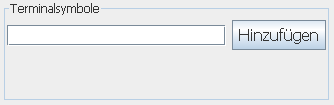
\includegraphics[scale=0.5]{\pfad ebnf/ebnfinput_addterminal.png} \hfill
						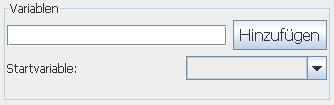
\includegraphics[scale=0.5]{\pfad ebnf/ebnfinput_addvariable.png} \\
						Eingabemaske f�r Terminalsymbole \hfill ...und f�r Variablen
					\end{center}
    			
	\end{itemize}

  \item Eingabe von Regeln \\

	Mit einer EBNF-Regel wird einer Variablen ein EBNF-Term zugeordnet. Die Variable kann
	aus der Drop-Down-Liste ausgew�hlt werden. Da es zu jeder Variablen nur eine Regel
	geben darf, werden nur diejenigen Variablen angezeigt, zu denen es noch keine Regel gibt.
	
	\begin{itemize}
    \item F�r einen korrekten EBNF-Term gelten folgende Regeln:
    
    \begin{itemize}
    	\item Ein EBNF-Term besteht aus Variablen, Terminalsymbolen und Metasymbolen
      \item Die Metasymbole m�ssen korrekt geklammert sein
      \item Der EBNF-Term darf nicht leer sein (genauso darf der in einer Klammerung
      			enthaltene Sub-Term nicht leer sein) 
    \end{itemize}
    
    \item Eine neue Regel kann mit der Eingabetaste oder Klick auf Hinzuf�gen zur
    			Definition hinzugef�gt werden. Falls die Regel nicht hinzugef�gt werden kann,
    			wird eine entsprechende Fehlermeldung angezeigt.
    			
    			\centerpic{ebnf/ebnfinput_addrule.png}{.5}{Eingabemaske f�r Regeln}
    			
    \item Kommt in der Regel ein unbekanntes Symbol vor, so wird ein Dialogfenster
    		  angezeigt, welches die M�glichkeit bietet, das neue Symbol der Menge der 
    		  Variablen oder Terminalsymbole hinzuzuf�gen. Man kann auch Teile des nicht 
    		  erkannten Textes als Symbol hinzuf�gen, indem man den Text im Dialog 
    		  bearbeitet. In diesem Fall ist es m�glich, dass weitere unbekannte Symbole 
    		  gefunden werden. W�hlt man in diesem Dialog �Abbrechen�, so schl�gt das 
    		  Hinzuf�gen der Regel fehl. 
    		  
    		  \centerpic{ebnf/ebnfinput_unknownsymbol.png}{.5}{Dialog f�r unbekannte Symbole}
    		  
  \end{itemize}
  
  \item Setzen der Startvariable

  \begin{itemize}
  
  	\item Eine Definition besitzt genau dann eine Startvariable, wenn sie mindestens eine 
  				Variable enth�lt. Beim Hinzuf�gen der ersten Variablen wird diese automatisch zur 
  				Startvariable.
  				
  				\centerpic{ebnf/ebnfinput_setstartvar.png}{.8}{Setzen der Startvariable}
  				
  				
    \item Die Startvariable kann ge�ndert werden, indem man eine Variable aus der 
    			entsprechenden Drop-Down-Liste ausw�hlt. Au�erdem kann man eine Variable �ber ihr 
    			Kontextmen� in der Anzeige der Variablenmenge als Startvariable setzen. 
    			
    			\centerpic{ebnf/ebnfinput_popup_startvar.png}{.8}{Setzen der Startvariable in der Ansicht}
	\end{itemize}

\end{itemize}

\subsubsection{Bearbeiten einer Definition}

M�chte man an einer bereits eingegebenen Definition �nderungen vornehmen, zum Beispiel eine Regel l�schen oder ein Terminalsymbol umbenennen, so kann dies �ber das Kontextmen� in der Ansicht geschehen.

\begin{itemize} 

	\item L�schen

	\begin{itemize} 
	
		\item L�schen von Variablen und Terminalsymbolen
	
  	\begin{itemize} 
  		\item Ein Symbol kann nur dann gel�scht werden, wenn es in keiner Regel mehr 
  					vorkommt.
    	\item Wenn dies der Fall ist, kann man im Kontextmen� des Symbols in der Variablen- 
    				oder Terminalsymbolmenge die Funktion "`L�schen"' ausw�hlen. 
    				
    				\centerpic{ebnf/ebnfinput_delvariable.png}{.8}{L�schen einer Variable}
    				
    				
    \end{itemize}
    
    \item L�schen von Regeln \\
    			Regeln k�nnen �ber das Kontextmen� in der Regel-Ansicht gel�scht werden. 
    			
    			\centerpic{ebnf/ebnfinput_delrule.png}{.8}{L�schen einer Regel}
  \end{itemize}

  \item Bearbeiten
  
  \begin{itemize} 
		\item Bearbeiten von Variablen und Terminalsymbolen.
		
    \begin{itemize} 
  		\item Symbole k�nnen �ber ihr Kontextmen� umbenannt werden. Dabei gelten f�r die 
  					Namens�nderung die gleichen Regeln wie f�r die Eingabe.
      \item W�hlt man im Kontextmen� eines Symbols �Bearbeiten� aus, so erscheint in der 
      			entsprechenden Eingabemaske das Symbol, der Hinzuf�gen-Button �ndert sich in 
      			einen ��ndern�-Button und es erscheint zus�tzlich ein �Abbrechen�-Button. Im 
      			Textfeld kann man den Symbolnamen �ndern und anschlie�end durch die Auswahl 
      			von ��ndern� �bernehmen. M�chte man die �nderung abbrechen, so kann man dies 
      			�ber den entsprechenden Button vornehmen.
      \item Grunds�tzlich kann man immer nur eine Variable und ein Terminalsymbol 
      			gleichzeitig bearbeiten; im Moment bearbeitete Symbole werden in der Ansicht 
      			gelb hervorgehoben. 
      			
      			\bigskip
      			
      			\centerpic{ebnf/ebnfinput_editvar.png}{.6}{Umbenennen einer Variable}
      			
      			\bigskip
      			
      			\centerpic{ebnf/ebnfinput_editterminal.png}{.6}{Umbenennnen eines Terminalsymbols}
      			
    \end{itemize}  			
    \bigskip  			
    \item Bearbeiten von Regeln
    
    \begin{itemize} 
			\item Regeln k�nnen �ber ihr Kontextmen� bearbeitet werden.
      \item W�hlt man im Kontextmen� einer Regel �Bearbeiten� aus, so erscheint in der 
      			Regel-Eingabemaske die Regel, der Hinzuf�gen-Button �ndert sich in einen 
      			��ndern�-Button und es erscheint zus�tzlich ein �Abbrechen�-Button. Im 
      			Textfeld kann man den Term bearbeiten und anschlie�end durch die Auswahl von 
      			��ndern� �bernehmen. Das �ndern der Variablen der Regel ist nicht m�glich. 
      			M�chte man die �nderung abbrechen, so kann man dies �ber den entsprechenden 
      			Button vornehmen.
      			
      			\bigskip
      			
      			\centerpic{ebnf/ebnfinput_editrule.png}{.6}{Bearbeiten einer Regel}
      			
      			\bigskip
      			
      \item Grunds�tzlich kann man immer nur eine Regel bearbeiten; die im Moment 
      			bearbeitete Regel wird in der Ansicht gelb hervorgehoben. 
    \end{itemize}
  \end{itemize}
\end{itemize}

\bigskip

\subsubsection{�berpr�fen einer Definition und Beenden der Eingabe}

Um eine Definition zu �berpr�fen kann der Button �Definition �berpr�fen� genutzt werden. Die Definition wird dann auf folgende Fehler und m�gliche Probleme �berpr�ft:

\begin{itemize}
	\item Das Vorhandensein einer Startvariable (--> Fehlermeldung)
	\item Das Vorhandensein einer Regel f�r jede Variable (--> Fehlermeldung)
	\item Die Nutzung aller Variablen der Variablenmenge (--> Warnung)
	\item Die Nutzung aller Terminalsymbole der Terminalsymbolmenge (--> Warnung)
	\item Die Erreichbarkeit aller Regeln von der Startvariablen aus (--> Warnung) 
\end{itemize}

Wird mind. ein Fehler gefunden, so werden Warnungen ignoriert und nicht angezeigt, um die �bersicht zu wahren. \\

Durch das Aktivieren des \textsc{Eingabe beenden}-Buttons wird die Definition �berpr�ft. Wird dabei mind. ein Fehler gefunden, so kann der Wechsel zur EBNF-Anzeige nicht stattfinden. Wenn kein Fehler auftritt (Warnungen k�nnen vorkommen, werden aber nicht angezeigt) geschieht ein Wechsel zur EBNF-Anzeige, in welcher die Eingabemaske nicht mehr zu sehen ist.
\subsection{Anzeige von EBNF-Defintionen}

Die EBNF-Anzeige kann nur erreicht werden, wenn die Definition korrekt und vollst�ndig ist. Eine �berpr�fung dessen findet durch die vorausgegangene Nutzung des \textsc{Eingabe beenden}-Buttons bzw. Beim Laden einer Datei statt. \\

Hintergrund der EBNF-Anzeige ist die �bersichtliche Anzeige einer EBNF-Definition, ohne die Eingabemaske. Au�erdem besteht hier die M�glichkeit, zum trans()-Algorithmus zu wechseln, um die EBNF-Definition in ein Syntaxdiagramm umzuwandeln. 

\subsubsection{Definition bin�r klammern}

Um in den trans()-Algorithmus wechseln zu k�nnen, muss die Definition bin�r geklammert sein. Nach strenger Auslegung der Definition existieren nur bin�re Alternativen in der EBNF: 
\begin{itemize}
	\item nicht bin�r geklammert: (a|b|c)
	\item korrekt geklammert: (a|(b|c))
\end{itemize}

\centerpic{ebnf/ebnfdisplay_makebinary.png}{.6}{Definition bin�r klammern}

\bigskip

Der Lesbarkeit halber erm�glicht das Programm eine Eingabe von nicht bin�r geklammerten Alternativen. Ob die Definition noch nicht korrekt geklammerte Terme enth�lt, wird durch eine entsprechende Meldung angezeigt: BILD \\

Um eine Definition bin�r zu klammern, muss der \textsc{Definition bin�r klammern}-Button genutzt werden. Dadurch werden die noch fehlenden Klammern hinzugef�gt und rot hervorgehoben. Damit ist der Wechsel zum trans()-Algorithmus erm�glicht. 

\subsubsection{Wechsel zum trans()-Algorithmus}

Wenn die Definition bin�r geklammert ist, kann man in den trans()-Algorithmus durch Anklicken des \textsc{trans()-Algorithmus anwenden}-Buttons wechseln.

\subsubsection{Beibehalten der bin�ren Klammerung}

Falls in der EBNF-Anzeige nachtr�glich eine bin�re Klammerung vorgenommen wurde, so wird beim Wechsel zur EBNF-Eingabe (mittels \textsc{Definition �berarbeiten}-Button) und beim Speichern aus der EBNF-Anzeige heraus nachgefragt, ob diese in der Definition beibehalten werden soll.

\bigskip
\centerpic{ebnf/ebnfdisplay_keepbinary.png}{.8}{Beibehalten der Klammerung}
\bigskip
\subsection{Speichern und Laden von EBNF-Defintionen}

Man kann grunds�tzlich Definitionen zu jedem Zeitpunkt in der EBNF-Eingabe speichern. \\

Dies geschieht entweder �ber das Men� \textsc{Datei} oder die ensprechenden Symbole in der Werkzeugleiste. Au�erdem wird gefragt, ob die Definition gespeichert werden soll, sobald man das Modul verlassen m�chte und nicht gesicherte Ver�nderungen vorgenommen hat. \\

Falls in der EBNF-Anzeige nachtr�glich eine bin�re Klammerung vorgenommen wurde, so wird beim Speichern aus der EBNF-Anzeige heraus nachgefragt, ob diese in der Definition beibehalten werden soll. \\

\newpage
\section{Der trans()-Algorithmus}

\subsection{\label{transArbeitsFlaeche}Die Arbeitsfl�che}


\bigskip
\centerpic{ebnf/trans_gui.png}{.4}{Die Arbeitsfl�che des trans()-Algorithmus}
\bigskip

\begin{itemize}
	\item Anzeigebereich \\
				Hier werden die Syntaxdiagramme visualisiert, vollst�ndig, sowie auch w�hrend des 
				Algorithmus. Neben den Syntaxdiagrammelementen existieren hier zus�tzlich noch die 
				hinterlegten trans()-Elemente. F�hrt man mit der Maus dar�ber, werden die zu 
				trennenden Elemente farblich hervorgehoben und im Erkl�rungsbereich wird der 
				dazugeh�rige Schritt angezeigt. Bei Klick, wird dieser Schritt ausgef�hrt.

  \item Kontrollbereich \\
  			Im Kontrollbereich hat man die M�glichkeit, die Syntaxdiagramme grafisch zu 
  			ver�ndern. Die M�glichkeiten beschr�nken sich auf das Skalieren der Diagramme, das 
  			automatische Anpassen der Gr��e an das Fenster, sowie die Entfernung von 
  			Treppenstrukturen. Auf der rechten Seite befinden sich zudem noch 
  			Navigationsbuttons.


	\begin{itemize}
		\item \icon{ebnf/trans_resize.png}{0}{0}{.6} Hier haben Sie die M�glichkeit, das Diagramm selbst zu 
					vergr��ern und zu verkleinern

		\item \icon{ebnf/trans_fit.png}{0}{0}{.6} Hier kann man einstellen, ob sich die Gr��e der Diagramme 
					automatisch dem Fensterrahmen anpassen soll oder nicht.

		\item \icon{ebnf/trans_stairs.png}{0}{0}{.6} Bei Aktivierung dieses Knopfes, werden Treppenstrukturen in 
					den Diagrammen entfernt.

		\item Wechsel zur Syntaxdiagramm-Anzeige \\
					ACHTUNG! Ein Wechsel in die Syntaxdiagramm-Anzeige ist nur nach Beendigen des 
					Algorithmus m�glich und man kommt zudem nicht wieder zur�ck! 
					
		\item Wechsel zur EBNF-Definition \\
					Wechselt man in die 
					Ebnf-Ansicht und l�sst die Ebnf-Definition unver�ndert, f�hrt man bei R�ckkehr in 
					den trans()-Algorithmus fort, �ndert man die Ebnf-Defintion, wird der Algorithmus 
					neu gestartet.

	\end{itemize}
	
  \item Steuerbereich \\
				Hier kann man neben dem direkten Arbeiten in der Anzeige noch �ber Buttons den 		
				Algorithmus steuern.

	\begin{itemize}
		\item \icon{ebnf/trans_reset.png}{0}{0}{.6} Macht alle bisher ausgef�hrten Schritte r�ckg�ngig

		\item \icon{ebnf/trans_last.png}{0}{0}{.6} Macht den letzten ausgef�hrten Schritt r�ckg�ngig

		\item \icon{ebnf/trans_info.png}{0}{0}{.6} Bei Aktivierung dieses Buttons wird permanent der n�chste Schritt 
					hervorgehoben

		\item \icon{ebnf/trans_next.png}{0}{0}{.6} F�hrt den n�chsten automatisch gew�hlten Schritt aus

		\item \icon{ebnf/trans_finish.png}{0}{0}{.6} F�hrt den Algorithmus bis zum Ende aus

	\end{itemize}
	
  \item Erkl�rungsbereich \\
				Hier werden die Erkl�rungen zu den einzelnen Schritten angezeigt oder es werden dem 
				Nutzer Hinweise angezeigt
\end{itemize}	
	
\subsection{Steuerung des Algorithmus}

Es existieren zwei M�glichkeiten, den Algorithmus zu steuern. Zum einen

\begin{itemize}
	\item Im Anzeigebereich \\
				Hier kann man direkt mit den farblich hinterlegten trans()-Elementen arbeiten. 			
				Befindet sich die Maus dar�ber, werden die zu trennenden Teilst�cke hervorgehoben 
				sowie der zugeh�rige Algorithmusschritt im Erkl�rungsbereich angezeigt. Klickt man 
				darauf, wird dieser Schritt ausgef�hrt und das Element umgeformt.

	\item �ber die Steuerbuttons \\
				Die Erkl�rung zu den Steuerbuttons befindet sich im Abschnitt 
				\ref{transArbeitsFlaeche} in der Erkl�rung zur Arbeitsfl�che.
\end{itemize}

\newpage
\section{Syntaxdiagramme}

\subsection{Der Syntaxdiagramm-Editor}

\subsubsection{Die Arbeitsfl�che}

Die Arbeitsfl�che des Syntaxdiagramm-Editors ist zweigeteilt: Im oberen Abschnitt befindet sich der Kontrollbereich, �ber den alle Aktionen, die f�r das Erstellen und Editieren von Syntaxdiagrammen n�tig sind, anw�hlbar sind. Darunter befindet sich die Anzeige f�r Syntaxdiagramme - die Arbeitsfl�che, auf der an den Diagrammen gearbeitet wird.

\bigskip
\centerpic{ebnf/syndia_aufteilung.png}{.4}{}
\bigskip

\subsubsection{Hinzuf�gen von Elementen}

Um einem Syntaxdiagrammsystem Elemente hinzuf�gen zu k�nnen, muss man sich in einem entsprechenden Modus befinden. Einzig das Hinzuf�gen neuer Syntaxdiagramme geschieht ohne Moduswechsel.

\begin{itemize}
	\item Syntaxdiagramme \\
				Um ein neues Syntaxdiagramm einzuf�gen gen�gt ein einfacher Klick auf das Symbol 
				\icon{ebnf/syndia_Leiste_NeuesDiagramm.png}{0}{0}{.4} im Kontrollbereich. In der Syntaxdiagramm-Anzeige erscheint ein 
				Popupfenster, in dem sich u.a. ein Texteingabefeld befindet. In diesem bereits 
				fokusierten Eingabefeld k�nnen Sie nun den gew�nschten Namen ihres neuen 
				Syntaxdiagramms angeben. Ihre Eingabe beenden Sie entweder mit dem OK-Button \icon{ebnf/syndia_Button_OK.png}{0}{0}{.4}
				rechts des Eingabefeldes oder �ber \textsc{Enter}. \\

				Falls der von Ihnen gew�hlte Name schon f�r ein anderes Diagramm vergeben ist, 
				werden Sie im Rahmentext des Popupfensters darauf hingewiesen. Sie m�ssen einen 
				anderen Namen w�hlen. \\

				Unterhalb des Eingabefeldes befindet sich eine weitere Zeile: 
				
\centerpic{ebnf/syndia_startdiagramm.png}{.8}{}

	
				Indem Sie die 
				Checkbox ausw�hlen, k�nnen Sie ihr neues Diagramm als Startdiagramm einf�gen. Es 
				ist immer nur ein Startdiagramm zul�ssig, d.h. das alte Startdiagramm verliert 
				dieses "`Privileg"' an das neue Syntaxdiagramm. \\

				Sie k�nnen die Eingabe jederzeit mit \textsc{Esc} abbrechen. Die Eingabe eines leeren 
				Diagrammnamens bewirkt ebenfalls einen Abbruch. Es wird kein Syntaxdiagramm 
				hinzugef�gt.

  \item �ber die Einf�ge-Modi \\
				Um Elemente einf�gen zu k�nnen, m�ssen Sie in den Modus "`<Element> einf�gen"' 
				wechseln. Dieses Beispiel demonstriert dies f�r Terminalsymbole. Den Moduswechsel 
				erreichen Sie auf zwei verschiedenen Wegen: entweder w�hlen Sie im Kontrollbereich 
				den Button \icon{ebnf/syndia_Leiste_Terminal.png}{0}{0}{.4} aus oder Sie bewegen Ihre Maus in die Syntaxdiagramm-Anzeige. 
				Dort k�nnen Sie jederzeit mit einem Rechtsklick ein Kontextmen� �ffnen, in dem Sie 
				ebenfalls den Modus "`Terminalsymbole einf�gen"' anw�hlen k�nnen. \icon{ebnf/syndia_Popup_Terminal.png}{0}{0}{.4} \\

				Ist dieser Modus gew�hlt, wird der zugeh�rige Button im Kontrollbereich ausgegraut. 
				Auch �ndert sich der Mauszeiger, wenn Sie �ber den Arbeitsbereich fahren. \\	
				
				Somit wissen Sie immer, in welchem Modus Sie sich gerade befinden.

  \item �ber die Rhomben \\
				Im Editiermodus bekommen die Syntaxdiagramme neue Elemente - die Rhomben. Sie sind 
				Pseudoelemente, die das Einf�gen von Elementen erleichtern bzw. erst erm�glichen. 
				In ihrem Grundzustand sind die Rhomben grau. Befindet man sich in einem 
				Einf�gemodus, so leuchten sie gr�n auf, falls an dieser Stelle ein Hinzuf�gen 
				m�glich ist. Leuchten sie dagegen rot auf, kann das Element an dieser 
				Stelle nicht eingef�gt werden. \\

				Hat man etwas eingef�gt, erscheinen vor und hinter diesem Element neue Rhomben, an 
				denen erneut hinzugef�gt werden kann. In Wiederholungen und Verzweigungen 
				erscheinen zudem in den Elementen neue Rhomben - schlie�lich soll man auch hier 
				Einf�gen k�nnen.

  \item Terminalsymbole und Variablen \\
				Wechseln Sie als erstes in den Modus \textsc{Terminalsymbole einf�gen} oder \textsc{Variablen einf�gen}. \icon{ebnf/syndia_Leiste_Terminal.png}{0}{0}{.4}\icon{ebnf/syndia_Leiste_Variable.png}{0}{0}{.4} In der Arbeitsfl�che k�nnen Sie nun mit der Maus �ber 
				jeden beliebigen Rhombus fahren - er leuchtet gr�n auf. Mit einem Linksklick f�gen 
				Sie das Terminalsymbol / die Variable an dem aktuell gr�n leuchtenden Rhobus ein. \\

				Es erscheint ein Textfeld, in dem Sie einen Namen f�r das Element eingeben m�ssen. 
				Als Standard erscheint ausgew�hlt "`a"' / "`A"'. \\

				Zum Best�tigen einer Eingabe dr�cken Sie entweder auf den OK-Button \icon{ebnf/syndia_Button_OK.png}{0}{0}{.4} oder 
				ENTER. Falls Sie das Erstellen abbrechen m�chten, dr�cken Sie ESACAPE oder geben 
				einen leeren Namen ein.

  \item Verzweigungen und Wiederholungen \newline
  			Wechseln Sie als erstes in den Modus "`Verzweigungen einf�gen"' / "`Wiederholungen 
  			einf�gen"' \icon{ebnf/syndia_Leiste_Verzweigung.png}{0}{0}{.4}\icon{ebnf/syndia_Leiste_Wiederholung.png}{0}{0}{.4}. In der Arbeitsfl�che k�nnen Sie nun mit der Maus �ber 
  			jeden beliebigen Rhombus fahren - er leuchtet gr�n auf. Mit einem Linksklick f�gen 
  			Sie den Anfang der Verzweigung / Wiederholung ein. Daraufhin erscheint grau 
  			gepunktet eine neue Verzweigung / Wiederholung. Diese zeigt, von wo bis wo 
  			eingef�gt werden kann. Anfangs ist sie auf den angeklickten Rhombus beschr�nkt. \\

				Sie k�nnen diese "`unfertige"' Verzweigung / Wiederholung nun sowohl nach links als 
				auch nach rechts in die Breite ziehen. Fahren Sie dazu mit der Maus �ber andere 
				Rhomben. Leuchtet ein Rhombus gr�n auf, so kann bis zu dieser Stelle eingef�gt 
				werden. Dies wird durch die ver�nderte grau gepunktete Verzweigunng / Wiederholung 
				angezeigt. Dabei k�nnen auch schon vorhandene Elemente eingeschlossen werden. \\

				Leuchtet ein Rhombus dagegen rot auf, so darf an dieser Stelle nicht eingef�gt 
				werden. Dies ist der Fall, wenn das Ende nicht auf der gleichen Linie liegt wie der 
				Startpunkt. Auch d�rfen sich Linien nicht kreuzen, so dass das Einf�gen eines Endes 
				in das Innere einer anderen Verzweigung / Wiederholung ebenfalls nicht erlaubt ist. 				\\

				Haben Sie den Mauszeiger �ber ein gr�n leuchtendes Ende gefahren, so k�nnen Sie nun 
				mit einem weiteren Linksklick Einf�gen. Die grau gepunktete Verzweigung / 
				Wiederholung verschwindet und ein vollst�ndig neues Element erscheint.
\end{itemize}

\subsubsection{Bearbeiten und L�schen von Elementen}

\begin{itemize}
	\item Editieren \\
				Im Editiermodus ist es m�glich, Terminalsymbol-, Variablen- und Syntaxdiagrammnamen 
				zu �ndern. \\

				Wechseln Sie dazu zuerst in diesen Modus. \icon{ebnf/syndia_Leiste_Edit.png}{0}{0}{.5} \\

Fahren Sie nun mit der Maus �ber Terminalsymbole oder Variablen, so leuchten diese blau auf. Mit einem Linksklick auf diese Elemente erscheint ein Textfeld mit dessen Namen. Sie k�nnen den Namen nun beliebig �ndern. Mit dem OK-Button oder \textsc{Enter} schlie�en Sie die �nderung ab. Mit \textsc{Escape} oder der Eingabe eines leeren Namens brechen Sie den Editiervorgang ab. \\

Fahren Sie mit der Maus �ber den Namen eines Syntaxdiagramms, so erscheint dieser fett. Mit einem Linksklick k�nnen Sie nun den Namen des Diagramms �ndern. Dazu erscheint der Dialog, der auch zum Einf�gen neuer Elemente angezeigt wird. Einziger Unterschied ist, dass, falls Sie das Startdiagramm editieren, Sie diesem Diagramm diesen Status nicht nehmen k�nnen - die entsprechende Checkbox ist ausgegraut.

	\item L�schen \\

Im L�schmodus ist es m�glich, sowohl alle Syntaxdiagrammelemente als auch leere Diagramme zu l�schen.

Wechseln Sie dazu zuerst in diesen Modus. \icon{ebnf/syndia_Leiste_Radiergummi.png}{0}{0}{.5} \\

Fahren Sie nun mit der Maus �ber Terminalsymbole oder Variablen, so leuchten diese rot auf. Mit einem Linksklick werden diese gel�scht. Nachfolgende Elemente r�cken nach links.

Verzweigungen und Wiederholungen k�nnen ebenfalls gel�scht werden. Bewegen Sie dazu den Mauszeiger auf die obere oder untere Linie eines dieser Elemente. Die Linie und alle darauf liegenden Elemente leuchten rot auf. Mit einem Linksklick best�tigen Sie den L�schvorgang.
War die untere Linie markiert, so werden Elemente der oberen Linie beibehalten. L�schen Sie die obere Linie einer Verzweigung, so werden die Elemente der unteren Linie - sofern vorhanden - auf die obere Linie eingef�gt. Die untere Linie verschwindet. Dies geschieht auch beim L�schen des unteren Teils einer Wiederholung; nur werden hier die Elemente in umgekehrter Reihenfolge oben eingef�gt (d.h. ihre "`Leserichtung"' bleibt erhalten). \\

Befinden Sie sich mit dem Mauszeiger �ber einem leeren Syntaxdiagramm (d.h. nur ein Rhombus befindet sich in diesem Diagramm), so erscheint um dieses ein roter Rahmen. Best�tigen Sie mit einem Linksklick, wird das Diagramm gel�scht. Handelt es sich dabei um das Startdiagramm, so erscheint ein Hinweis, dass das L�schen des Startdiagramms nicht m�glich ist.

\end{itemize}
\subsection{Die Syntaxdiagramm-Anzeige}

\bigskip
\centerpic{ebnf/syndia_view.png}{.4}{}
\bigskip

\subsubsection{Anzeigebereich}

Hier werden die Syntaxdiagramme visualisiert.

\subsubsection{Kontrollbereich}

Im Kontrollbereich hat man die M�glichkeit, die Syntaxdiagramme grafisch zu ver�ndern. Die M�glichkeiten beschr�nken sich auf das Skalieren der Diagramme, das automatische Anpassen der Gr��e an das Fenster, sowie das Entfernen von Treppenstrukturen. Auf der rechten Seite befinden sich zudem noch Navigationsbuttons.

	\begin{itemize}
		\item \icon{ebnf/trans_resize.png}{0}{0}{.6} Hier haben Sie die M�glichkeit, das Diagramm selbst zu 
					vergr��ern und zu verkleinern

		\item \icon{ebnf/trans_fit.png}{0}{0}{.6} Hier kann man einstellen, ob sich die Gr��e der Diagramme 
					automatisch dem Fensterrahmen anpassen soll oder nicht.

		\item \icon{ebnf/trans_stairs.png}{0}{0}{.6} Bei Aktivierung dieses Knopfes, w�hrend Treppenstrukturen in 
					den Diagrammen entfernt.

	\end{itemize}
\subsection{Speichern und Laden von Syntaxdiagrammen}

\subsubsection{Speichern}

Nat�rlich haben Sie auch die M�glichkeit, Syntaxdiagramme zu speichern. \\

Dies ist m�glich in der Syntaxdiagramm-Anzeige sowie im Syntaxdiagramm-Editor. Das Speichern ist nur mit der Endung \emph{"`*.jalgo"'} m�glich. Das Programm erkennt jedoch automatisch, dass es sich um ein Syntaxdiagramm handelt. \\

Hinweis! Speichern sie die Diagramme in einem eindeutigen Ordner oder geben Sie dem Diagramm einen geeigneten Namen, da die Speicherendungen im gesamten \jalgo \emph{"`*.jalgo"'} sind.

\subsubsection{Laden von Syntaxdiagrammen}

Beim Laden von Syntaxdiagrammen unterscheidet das Modul, ob sie vollst�ndig sind oder nicht. Vollst�ndig bedeutet, dass zu jeder Variable im Diagramm ein Diagramm mit diesem Namen existiert. Ist es vollst�ndig, befinden Sie sich nach dem Laden in der Syntaxdiagrammanzeige. Ist es nicht vollst�ndig wird der Editor ge�ffnet und das Diagramm kann bearbeitet werden. 

\newpage
\section{Der R�cksprung-Algorithmus}

\subsection{Die Arbeitsfl�che}

Die Arbeitsfl�che des R�cksprungalgorithmus ist in vier Bereiche aufgeteilt.


\bigskip
\centerpic{ebnf/rs_full.png}{.8}{Der R�cksprungalgorithmus}
\bigskip

\begin{itemize}
	\item Syntaxdiagramm-Ansicht \\
				die Syntaxdiagramme werden hier grafisch dargestellt. Dar�ber hinaus erfolgt die 
				Steuerung w�hrend des Algorithmus� durch Anklicken der Diagramme in dieser Ansicht.

  \item Keller \\
				Hier werden alle R�cksprungadressen dargestellt, die w�hrend des Algorithmus� auf 
				den Keller gelegt werden.

  \item Kontrollbereich \\
				Hier wird das Wort ausgegeben, das w�hrend des Algorithmus� erzeugt wurde. Dar�ber 
				hinaus kann hier ein Wort eingegeben werden, das erzeugt werden soll, der 
				Algorithmus wird von hier gestartet. Zus�tzlich bietet der Kontrollbereich die 
				M�glichkeit, die Darstellung der Syntaxdiagramme in der Syntaxdiagramm-Ansicht 
				anzupassen.

  \item Erkl�rungsbereich  \\
  			Hier werden w�hrend des Ablaufes des Algorithmus� Erkl�rungen zu den einzelnen 
  			Algorithmusschritten ausgegeben. 
\end{itemize}

\subsection{Steuerung des Algorithmus}

Aufgabe des Bereichs �R�cksprungalgorithmus� ist es, den Algorithmus der Worterzeugung zu visualisieren. Er repr�sentiert den Ablauf eines Weges durch ein Syntaxdiagramm-System und erzeugt w�hrend des Ablaufes ein Wort, das sich aus den passierten Terminalsymbolen zusammensetzt. Das Modul ist dabei nicht in der Lage, Entscheidungen �ber die Wegewahl bez�glich der Erzeugung eines Wortes selbst zu treffen. Vielmehr soll er dem Nutzer helfen, eigene Durchl�ufe und Spr�nge zwischen den einzelnen Diagrammen zu �berpr�fen.

Im Folgenden wird die Steuerung des Algorithmus� erl�utert:

\subsubsection{Eingabe eines Wortes}

Bevor der Algorithmus gestartet wird, besteht die M�glichkeit, im Kontrollbereich ein Wort einzugeben, welches w�hrend des Algorithmus erzeugt werden soll. Dieses kann einfach in das Textfeld eingegeben werden, welches mit �Zu erzeugendes Wort� bezeichnet ist. Die Eingabe eines Wortes, welches erzeugt werden soll, ist optional. Es ist genauso m�glich, kein Wort einzugeben und die Generierung von W�rtern so zu testen, oder den Button 'Wort erzeugen' im Kontrollbereich zu klicken, der automatisch ein Wort - welches auch mit dem Algorithmus erzeugt werden kann - generiert (Dabei kann es sich aber auch um das leere Wort handeln, falls das Syntax-Diagramm-System dieses erm�glicht).

\subsubsection{Start des Algorithmus}

Nach der (optionalen) Eingabe eines Wortes kann der Algorithmus gestartet werden. Dies ist �ber einen Klick auf den Button �Algorithmus starten� im Kontrollbereich, oder �ber das Men� R�cksprung-Algorithmus-> Algorithmus starten m�glich.

Anmerkung: Besteht das im Schritt 1 eingegebene Wort nicht ausschlie�lich aus in den Syntax-Diagrammen vorhandenen Terminalsymbolen, so ist die Erzeugung eines solchen Wortes prinzipiell nicht m�glich. Das Programm wird ein solches Wort zur�ckweisen und den Algorithmus nicht starten.

Ist der Algorithmus gestartet, so wird die aktuelle Position in einem der gegebenen Programme durch einen roten Punkt gekennzeichnet. 


\bigskip
\centerpic{ebnf/rs_dot.png}{.8}{}
\bigskip

Zu Beginn des Algorithmus wird dieser Punkt am Anfang des Startdiagrammes stehen.

\subsubsection{W�hlen eines Weges durch ein Syntax-Diagramm}

Um einen Weg durch ein Syntax-Diagramm zu w�hlen, k�nnen einzelne Elemente des Diagrammes in der Syntax-Diagramm-Anzeige direkt angeklickt werden. Folgende Elemente k�nnen angeklickt werden: Erreichbare Terminalsymbole und Variable, erreichbare und leere Verzweigungen sowie erreichbare Ausg�nge von Syntax-Diagrammen.

\subsubsection{Passieren eines Terminalsymboles}

Um ein Terminalsymbol zu passieren, kann dieses einfach angeklickt werden. Dies ist nur m�glich, wenn das entsprechende Terminalsymbol von der aktuellen Position im Syntax-Diagramm zu erreichen ist. Ist ein Terminalsymbol zu erreichen, so wird es blau hervorgehoben, sobald man mit der Maus �ber das Symbol f�hrt. Passierte Terminalsymbole werden an das Ende des erzeugten Wortes im Kontrollbereich angeh�ngt.

\bigskip
\centerpic{ebnf/rs_terminal.png}{.8}{}
\bigskip

\subsubsection{Passieren einer Variable}

Um eine Variable zu passieren, kann diese einfach angeklickt werden. Dies ist nur m�glich, wenn die entsprechende Variable von der aktuellen Position im Syntax-Diagramm zu erreichen ist. Ist eine Variable zu erreichen, so wird sie blau hervorgehoben, sobald man mit der Maus �ber die Variable f�hrt. Wird eine Variable passiert, so wird ihre R�cksprungadresse auf den Keller gelegt. Dem Passieren einer Variable folgt stets ein Sprung in ein Syntax-Diagramm.

\bigskip
\centerpic{ebnf/rs_variable.png}{.8}{}
\bigskip

\subsubsection{Sprung in ein Syntax-Diagramm}

Dem Sprung in ein Syntax-Diagramm geht stets das Passieren einer Variable voraus. Um in ein Syntax-Diagramm zu springen, muss einfach mit der Maus �ber das entsprechende Syntax-Diagramm in der Syntaxdiagramm-Ansicht gefahren werden, dieses wird dann mit einem blauen Rahmen umrandet. Durch den Klick auf das Diagramm wird der Sprung ins Diagramm durchgef�hrt. Ein Sprung ist nur m�glich, wenn der Name des Diagrammes, mit dem Inhalt der zuvor passierten Variable �bereinstimmt. Andernfalls wird der Algorithmus den Sprung zur�ckweisen.

\bigskip
\centerpic{ebnf/rs_frame.png}{.8}{}
\bigskip

\subsubsection{Passieren einer leeren Verzweigung}

Um eine leere Verzweigung zu passieren, kann diese einfach angeklickt werden. Dies ist nur m�glich, wenn die entsprechende Verzweigung von der aktuellen Position im Syntax-Diagramm zu erreichen ist. Ist eine leere Verzweigung zu erreichen, so wird sie blau hervorgehoben, sobald man mit der Maus �ber die Variable f�hrt. Beim Klick auf eine leere Verzweigung wird das erzeugte Wort nicht ver�ndert. Es �ndert sich lediglich die Position im Syntax-Diagramm.

\bigskip
\centerpic{ebnf/rs_mouseoverline.png}{.8}{}
\bigskip

\subsubsection{Verlassen eines Syntax-Diagrammes}

Ist nach dem Passieren eines Terminalsymboles, einer Variable oder leeren Verzweigung, sowie dem R�cksprung in ein Syntax-Diagramm nur noch der Ausgang des Diagrammes zu erreichen, so wird der Algorithmus das Diagramm automatisch verlassen. Doch nicht immer ist der Weg zum Ausgang die einzige M�glichkeit. In solchen Situationen muss man selbst entscheiden, ob das Diagramm verlassen werden soll. \\

Um das Diagramm zu verlassen, muss einfach in der Syntaxdiagramm-Anzeige auf den Ausgang des Diagrammes geklickt werden. Das Verlassen des Diagrammes wird nur durchgef�hrt, wenn der Ausgang des Diagrammes von der aktuellen Position im Diagramm erreicht werden kann. Der Ausgang des Diagrammes wird dann beim Fahren mit der Maus �ber den Ausgang blau hervorgehoben. \\

\bigskip
\centerpic{ebnf/rs_mouseoverexit.png}{.8}{}
\bigskip

Dem Verlassen des Diagrammes folgt entweder der R�cksprung in ein Diagramm, oder das Ende des Algorithmus. \\

\subsubsection{R�cksprung in ein Syntax-Diagramm}

Wurde ein Syntax-Diagramm verlassen, so kann ein R�cksprung in ein Diagramm folgen. Der R�cksprung folgt immer dann, wenn noch R�cksprungadressen auf dem Keller liegen. Um einen R�cksprung durchzuf�hren, muss einfach in der Syntaxdiagramm-Anzeige die R�cksprungmarke einer Variable in einem Diagramm angeklickt werden. Diese werden, falls ein R�cksprung m�glich ist, beim Fahren mit der Maus �ber die Marke blau hervorgehoben.

\bigskip
\centerpic{ebnf/rs_keller.png}{.8}{}
\bigskip

Ein R�cksprung wird nur durchgef�hrt, wenn die Nummer der angeklickten R�cksprungmarke mit der obersten Adresse auf dem Keller �bereinstimmt. Die oberste Adresse wird dann vom Keller gel�scht, der Weg kann hinter der Variable fortgesetzt werden, zu der zur�ckgesprungen wurde. Stimmen R�cksprungmarke und oberste Adresse auf dem Keller nicht �berein, so wird der R�cksprung vom Algorithmus zur�ckgewiesen.

\bigskip
\centerpic{ebnf/rs_variable_keller.png}{.8}{}
\bigskip

\subsubsection{Ende des R�cksprungalgorithmus}

Wird ein Syntax-Diagramm verlassen und es befindet sich keine R�cksprung-Adresse mehr auf dem Keller, so endet der Algorithmus. Er endet jedoch nur dann erfolgreich, wenn das Ende des Startdiagrammes erreicht wurde, und das vor Beginn des Algorithmus eingegebene Wort erzeugt wurde. Andernfalls wird der Algorithmus mit einer Fehlermeldung enden.

\subsubsection{Fehler w�hrend des Algorithmusdurchlaufes}

Nicht immer werden Fehler w�hrend des Laufens durch ein Syntax-Diagramm sofort erkannt und vom Algorithmus zur�ckgewiesen. So kann es z.B. passieren, dass das eingegebene Wort komplett erzeugt, der Ausgang des Startdiagrammes aber noch nicht erreicht wurde. Genauso kann ein anderes Wort als die Eingabe erzeugt worden sein. In einem solchen Fall wird der Algorithmus die Weiterarbeit verweigern. Es bestehen die M�glichkeiten, einzelne, falsche Schritte r�ckg�ngig zu machen, oder den Algorithmus komplett zur�ck zu setzen.

\subsubsection{Schritte r�ckg�ngig machen}

Um einen Schritt im Algorithmus r�ckg�ngig zu machen, gibt es zwei M�glichkeiten. Zum einen den Klick auf das entsprechende Symbol in der Toolbar am oberen Fensterrand \icon{ebnf/undo.png}{0}{0}{.5}, oder die Auswahl �ber das Men� R�cksprung-Algorithmus -> Schritt r�ckg�ngig.

\subsubsection{Schritte wiederherstellen}

Um einen Schritt im Algorithmus wiederherzustellen, gibt es zwei M�glichkeiten. Zum einen den Klick auf das entsprechende Symbol in der Toolbar am oberen Fensterrand \icon{ebnf/redo.png}{0}{0}{.5}, oder die Auswahl �ber das Men� R�cksprung-Algorithms -> Schritt wiederherstellen.

\subsubsection{Den R�cksprungalgorithmus zur�cksetzen}

Der Klick auf den Button \textsc{Algorithmus zur�cksetzen} im Kontrollbereich erm�glicht das Zur�cksetzen des Algorithmus in die Ausgangsposition. Einzelne Schritte k�nnen von hier aus wieder hergestellt werden. Es kann aber auch ein neues Wort eingegeben und der Algorithmus neu gestartet werden.

\subsubsection{Verlassen des R�cksprungalgorithmus-Bereiches}

Der R�cksprungalgorithmus-Bereich kann �ber den Button \textsc{Zur Syntaxdiagrammanzeige wechseln} im Kontrollbereich verlassen werden. Das Programm kehrt dann in die Syntaxdiagramm-Anzeige zur�ck. Die gleiche Funktionalit�t bietet die Auswahl im Men� R�cksprung-Algorithmus -> Algorithmus verlassen. 

\newpage

\section{Impressum}
Das Modul KMP wurde im Sommersemester 2006 von der Praktikumsgruppe SWT06-13 im Rahmen des externen Softwarepraktikums entwickelt. Mitwirkende waren die
\paragraph{Teammitglieder}
\begin{itemize}
	\item Danilo Lisske --- Chefprogrammierer
	\item Sebastian Patschorke  --- Assistent
	\item Matthias Neubert --- Testverantwortlicher
	\item 	Elisa B�hl --- Sekret�r
	\item Nadine Grabow --- Administrator
\end{itemize}
sowie der betreuende Tutor Matthias Schmidt.\\
Die Webseite des Projektes finden Sie unter \href{http://web.inf.tu-dresden.de/~swt06-13/}{http://web.inf.tu-dresden.de/\~{}swt06-13/}.

Das Handbuch zu diesem Modul wurde erstellt von Nadine Grabow.

\begin{appendix}
\newtheorem{alg}{Algorithmus}

\chapter{\label{appendix_avl_A}Einleitung zu Datenstrukturen}
\begin{tabbing}
\textbf{Anmerkung:} \=Der Autor der folgenden Seiten (Kapitel \ref{appendix_avl_A}, \ref{appendix_avl_B} und \ref{appendix_avl_C} dieses Anhangs) ist\\
\> Jean Christoph Jung (Teammitglied AVL-Modul)
\end{tabbing}

Eine h�ufige Anwendung auf gro�en Datenmengen ist das Suchen: Das Wiederfinden eines bestimmten Elements oder bestimmter Informationen aus einer gro�en Menge fr�her abgelegter Daten. Um die Suche zu vereinfachen, werden den (m�glicherweise sehr komplexen) gro�en Datens�tzen eineindeutige Suchschl�ssel (Keys) zugeordnet. Der Vergleich zweier solcher Schl�ssel ist in der Regel viel schneller als der Vergleich zweier Datens�tze. Wegen der Schl�sselzuordnung reicht es aus, alle vorkommenden Algorithmen nur auf den Schl�sseln zu betrachten; in Wirklichkeit verweisen erst die Schl�ssel auf die Datens�tze.\\
Eine grundlegende Idee ist nun, die Daten in Form einer Liste oder eines Feldes abzulegen. Diese Datenstruktur ist h�chst einfach. Jedoch ist der Aufwand f�r das Suchen relativ hoch, n�mlich $O(n)$. Genauer gesagt ben�tigt man f�r eine erfolglose Suche $n$ Vergleiche (bei $n$ Elementen in der Datenstruktur), denn man muss jedes Element �berpr�fen, und f�r eine erfolgreiche Suche durchschnittlich $(n+1)/2$ Vergleiche durchf�hren, da nach jedem Element mit der gleichen Wahrscheinlichkeit gesucht wird.\\
Eine Verbesserung dieses Verfahrens w�re, die Daten sortiert abzulegen, was zu einer bin�ren Suche f�hrt. Die Suche hat jetzt nur noch Komplexit�t $O(\log_2{n})$, da bei jedem Suchschritt das Feld halbiert wird. Der Nachteil ist, dass durch die Sortierung das Einf�gen erschwert wird, da unter Umst�nden viele Datens�tze bewegt werden m�ssen. Das Verfahren sollte also nur angewandt werden, wenn sehr wenige oder gar keine Einf�geoperationen ausgef�hrt werden m�ssen. Dann k�nnen die Daten anfangs mit einem schnellen Verfahren sortiert werden und m�ssen danach nicht mehr ver�ndert werden.\\
Eine weitere Datenstruktur, die der Suchb�ume, wollen wir hier vorstellen.

\chapter{\label{appendix_avl_B}Suchb�ume}
Suchb�ume sind bin�re B�ume (jeder Knoten hat h�chstens 2 Kinder) mit der Eigenschaft:\\
F�r jeden Knoten gilt: alle Schl�ssel im rechten Teilbaum sind gr��er als der eigene Schl�ssel und alle Schl�ssel im linken Teilbaum sind kleiner. Diese Eigenschaft wird hier immer Suchbaumeigenschaft genannt.

\centerpic{avl/bsp_suchbaum}{4.5}{Ein Beispiel f�r einen Suchbaum} 

An dieser Stelle noch eine Bemerkung zu den Schl�sseln: Die Schl�ssel k�nnen Elemente einer beliebigen Menge sein, unter der Bedingung, dass auf dieser Menge eine Ordnungsrelation definiert ist. Die Ordnungsrelation wird offensichtlich f�r die Suchbaumeigenschaft ben�tigt, da dort die Begriffe "`kleiner"' und "`gr��er"' vorkommen. Eine h�ufig verwendete Menge sind die nat�rlichen Zahlen mit ihrer normalen Ordnungsrelation $\leq$. Alle Operationen auf Suchb�umen kann man sich also anhand der nat�rlichen Zahlen vorstellen.\\
Aus der Suchbaumeigenschaft kann man sich leicht rekursive Algorithmen f�r das Einf�gen und Suchen in einem Suchbaum herleiten:

\begin{alg} \label{search}
	(Suchen eines Schl�ssels $s$ in einem Suchbaum)
	\begin{enumerate}
		\item Falls Teilbaum leer, dann Schl�ssel nicht im Baum vorhanden
		\item Falls $s$ gleich dem Schl�ssel des aktuellen Knoten, dann Suche erfolgreich.
		\item Falls $s$ gr��er als Schl�ssel des aktuellen Knotens, dann suche (rekursiv) $s$ im rechten Teilbaum.
		\item Falls $s$ kleiner als Schl�ssel des aktuellen Knotens, dann suche (rekursiv) $s$ im linken Teilbaum.
	\end {enumerate}
\end{alg}

\newpage
\begin{alg} \label{insert}
	(Einf�gen eines Schl�ssels $s$ in einen Suchbaum)
	\begin {enumerate}
		\item Falls Teilbaum leer, dann neuen Schl�ssel hier einf�gen.
		\item Falls $s$ gleich dem Schl�ssel des aktuellen Knotens, dann Schl�ssel bereits vorhanden, Einf�gen nicht n�tig.
		\item Falls $s$ gr��er als Schl�ssel des aktuellen Knotens, dann f�ge (rekursiv) $s$ in den rechten Teilbaum ein.
		\item Falls $s$ kleiner als Schl�ssel des aktuellen Knotens, dann f�ge (rekursiv) $s$ in den linken Teilbaum ein.
	\end {enumerate}
\end{alg}

Mit Algorithmus \ref{insert} ergibt sich folgende Eigenschaft der Struktur von Suchb�umen: im Gegensatz zur sortierten Liste h�ngt die Struktur eines Baumes davon ab, in welcher Reihenfolge die Elemente eingef�gt werden. So erh�lt man verschiedene B�ume, wenn man $1, 2, 3, 4$ in dieser Reihenfolge und in der Reihenfolge $3, 2, 4, 1$ einf�gt.

\centerpic{avl/12345}{4}{Unterschiedliche Suchb�ume bei unterschiedlicher Einf�gereihenfolge} 

Im ersten Fall erh�lt man einen Suchbaum, der zur linearen Liste entartet ist. Das ist nicht nur in dieser speziellen Reihenfolge so, es gibt viele M�glichkeiten einen entarteten Baum zu erzeugen. Der Algorithmus hat also zwei Nachteile: zum einen kann der Suchaufwand linear zur Anzahl der Knoten im Baum sein, was keine Verbesserung zur linearen Liste darstellt; zum anderen h�ngt die G�te des Verfahrens von der Eingabefolge ab. Der Vorteil von Suchb�umen wird klar, wenn man einen "`vollen"' Baum betrachtet, d.h. alle Pfade zu Bl�ttern haben dieselbe L�nge. Dann hat sowohl das Suchen (unabh�ngig davon, ob der Schl�ssel im Baum vorhanden ist) als auch das Einf�gen eine Komplexit�t von $O(\log{n})$.

\centerpic{avl/vollerbaum}{5}{Ein Beispiel f�r einen vollen Baum}
\medskip
Es gibt einige Algorithmen, bei denen der Einf�gealgorithmus so modifiziert ist, dass die entarteten F�lle vermieden werden und immer nahezu volle B�ume entstehen. Einen davon, den Algorithmus nach Adelson-Velskij und Landis (AVL), werden wir sp�ter betrachten.

Doch zun�chst wollen wir noch eine weitere wichtige Operation auf Suchb�umen untersuchen: das L�schen. Leider ist es nicht ganz so einfach wie Suche und Einf�gen.\\
Zuerst muss der zu l�schende Schl�ssel gesucht werden. Ist der betreffende Knoten ein Blatt, kann er einfach entfernt werden. Hat der zu l�schende Knoten nur ein Kind, kann er durch dieses ersetzt werden. Der schwierige Fall ist, wenn er zwei Kinder hat. Damit die Suchbaum\-eigenschaft erhalten bleibt, muss man ihn durch den n�chst gr��eren Schl�ssel ersetzen. Der n�chst gr��ere Schl�ssel befindet sich offensichtlich im rechten Teilbaum.

\centerpic{avl/remove}{5}{L�schen eines Knoten im Suchbaum}
\medskip
Nach dem Ersetzen bleibt die Suchbaumeigenschaft erhalten, weil alle Schl�ssel aus dem linken Teilbaum ohnehin kleiner sind als die aus dem rechten. Au�erdem sind auch alle Schl�ssel aus dem rechten Teilbaum gr��er, sonst w�re es nicht der n�chst gr��ere Schl�ssel gewesen. Aus diesen �berlegungen erh�lt man folgende verbale Beschreibung des L�schen-Algorithmus:

\newpage
\begin{alg} \label{delete}
	(L�schen eines Schl�ssels $s$ aus einem Suchbaum)
	\begin{enumerate}
		\item Suche s nach Algorithmus \ref{search}. Falls s nicht im Baum enthalten, terminiert der Algorithmus.
		\item \begin{enumerate}
			\item Ist der zu l�schende Knoten ein Blatt, dann entferne ihn einfach aus dem Baum.
			\item Hat der zu l�schende Knoten nur ein Kind, dann ersetze ihn durch dieses.
			\item Sonst suche den kleinsten Schl�ssel im rechten Teilbaum: Gehe zum rechten Kind und dann immer zum linken Teilbaum, solange dieser nicht leer ist. Ersetze den zu l�schenden Schl�ssel durch den des so gefundenen Knotens. Ersetze den gefundenen Knoten durch sein rechtes Kind.
			\end{enumerate}
	\end{enumerate}
\end{alg}

Man kann anstelle des n�chst gr��eren Schl�ssels genausogut den n�chstkleineren nehmen, der Algorithmus funktioniert trotzdem. Zur Komplexit�t ist zu sagen, dass der Algorithmus maximal $h$ Vergleiche macht, wobei $h$ die H�he des Baumes ist. Auch hier ist also die Komplexit�t abh�ngig von der Struktur des Baumes.

\chapter{\label{appendix_avl_C}AVL-B�ume}
AVL-B�ume (benannt nach Adelson-Velskij und Landis) sind spezielle Suchb�ume: In jedem Knoten unterscheiden sich die H�hen des linken Teilbaums und des rechten Teilbaums um h�chstens 1. Um diese Eigenschaft (AVL-Eigenschaft) abzusichern, wird f�r jeden Knoten ein Balancefaktor eingef�hrt. Der Balancefaktor ist die Differenz der H�hen des rechten Teilbaums und des linken Teilbaums. Also gilt f�r jeden AVL-Baum, dass alle Balancefaktoren aus $\{-1,0,1\}$ sind. B�ume mit AVL-Eigenschaft sind niemals als lineare Liste entartet (sofern sie denn mehr als 2 Knoten haben), sondern sind immer fast vollst�ndig. Zwischen der H�he $h$ eines Baumes und der Anzahl $n$ seiner Knoten besteht folgender Zusammenhang: $h\leq 2 \cdot \log_2{n}$. Das bedeutet, dass f�r das Suchen logarithmische Komplexit�t garantiert werden kann (das Suchen erfolgt gem�� Algorithmus \ref{search}).

\centerpic{avl/avlbsp}{5}{Ein Beispiel f�r einen AVL-Baum mit Balancen}
\medskip
Jetzt muss noch untersucht werden, wie gro� der zus�tzliche Aufwand beim Einf�gen ist, um die AVL-Eigenschaft zu wahren. In jedem Fall wird der neue Knoten als Blatt eingef�gt (nach demselben Algorithmus wie bei Suchb�umen). Dabei kann sich der Balancefaktor �ndern. Allerdings kann man sich leicht klarmachen, dass das nur entlang des Suchpfades passieren kann. Die Aktualisierung von Balancefaktoren erfolgt von der Einf�gestelle zur Wurzel. Hier der Algorithmus:

\newpage
\begin{alg} \label{avlinsert}
	(Algorithmus zum Einf�gen eines Elements x in einen AVL-Baum)
	\begin{enumerate}
		\item F�ge das neue Element x als direkten Nachfolger des Knotens n als Blatt ein, sodass die Suchbaumeigenschaft erf�llt bleibt. Aktualisiere n.balance.
		\item Setze n auf den Vorg�ngerknoten von n.
			\begin{enumerate}
				\item Falls x im linken Unterbaum von n eingef�gt wurde
					\begin{enumerate}
						\item wenn n.balance==1 dann n.balance=0 und gehe nach 3.
						\item wenn n.balance==0, dann n.balance=-1 und gehe nach 2.
						\item wenn n.balance==-1 und 
							\begin{itemize}
								\item wenn n.left.balance==-1, dann Rechts(n)-Rotation.
								\item wenn n.left.balance==1 dann Links(n.left)-Rechts(n)-Rotation.
							\end{itemize}
							Gehe zu 3.
					\end{enumerate}
				\item Falls x im rechten Unterbaum von n eingef�gt wurde
					\begin{enumerate}
						\item wenn n.balance==-1 dann n.balance=0 und gehe nach 3.
						\item wenn n.balance==0, dann n.balance=1 und gehe nach 2.
						\item wenn n.balance==1 und
							\begin{itemize}
								\item wenn n.left.balance==1, dann Links(n)-Rotation.
								\item wenn n.left.balance==-1 dann Rechts(n.left)-Links(n)-Rotation.
							\end{itemize}
							Gehe zu 3.
					\end{enumerate}
			\end{enumerate}
		\item Gehe zur�ck zur Wurzel.
	\end{enumerate}
\end{alg}

Zur Analyse dieses Algorithmus: Das reine Einf�gen erfolgt gem�� Einf�gen im Suchbaum (Algorithmus \ref{insert}), allerdings ist hier sichergestellt, dass sich die H�he logarithmisch zur Anzahl der Knoten verh�lt, d.h. auch der Aufwand f�r das Einf�gen ist garantiert logarithmisch. Wie gesagt k�nnen sich jedoch Balancefaktoren ge�ndert haben, sodass die AVL-Eigenschaft nicht mehr erf�llt ist. Das wird durch sogenannte Rotationen behoben. Es gibt zwei Typen von Rotationen -- Linksrotation und Rechtsrotation, jeweils um einen Knoten n.

\centerpic{avl/rotateleft}{5}{Linksrotation um den Knoten 65}  \medskip
\centerpic{avl/rotateright}{5}{Rechtsrotation um den Knoten 58}  \medskip

Falls durch das Einf�gen irgendwo ein Balancefaktor $2$($-2$) entsteht (gr��ere �nderungen k�nnen beim Einf�gen eines Knotens offensichtlich nicht auftreten), hei�t das, dass sich im rechten (linken) Teilbaum die H�he um 1 erh�ht hat. Durch Rotation(en) wie im Algorithmus angegeben, wird aber genau diese H�he wieder reduziert. Somit ist klar, dass man maximal zweimal rotieren muss, der Aufwand ist also noch ertr�glich, im Gegensatz zum L�schen, wie man gleich sehen wird.

Genauso wie Einf�gen ver�ndert auch L�schen eines Knotens aus einem AVL-Baum die Balancefaktoren, also m�ssen auch hier Rotationen ausgef�hrt werden. Hier der Algorithmus:

\begin{alg} \label{avldelete}
	L�schen eines Knotens aus einem AVL-Baum)
	\begin{enumerate}
		\item L�sche den Knoten analog zum L�schen im Suchbaum (Algorithmus \ref{delete}). Falls der Knoten ein Blatt war oder nur einen linken Nachbarn hatte, setze aktuellen Knoten auf den Vater. Sonst setze aktuellen Knoten auf den Vater des Knotens mit dem n�chst gr��eren Schl�ssel.
		\item Berechne den Balancefaktor des aktuellen Knotens neu. Falls
			\begin{enumerate}
				\item Balance 2 und rechte Balance -1, dann Rechts(n.right)-Links(n)-Rotation.
				\item Balance 2 und rechte Balance nicht -1, dann Links(n)-Rotation.
				\item Balance -2 und linke Balance 1, dann Links(n.left)-Rechts(n)-Rotation.
				\item Balance -2 und linke Balance nicht 1, dann Rechts(n)-Rotation.
				\item sonst keine Rotation.
			\end{enumerate}
			Wiederhole diesen Schritt solange, bis die Wurzel erreicht ist.
	\end{enumerate}
\end{alg}

Auch hier wollen wir den Aufwand des Algorithmus etwas genauer untersuchen. Schritt 1 entspricht dem L�schen aus dem Suchbaum, nur garantiert mit logarithmischen Aufwand. Die Frage ist nun, ob, wie beim Einf�gen, der Algorithmus mit maximal zwei Rotationen auskommt. Leider ist das nicht der Fall. Das liegt an der erw�hnten Eigenschaft der Rotationen, sie verringern die H�he eines Teilbaums. Beim Einf�gen war das gut, da durch das Anh�ngen eines Knotens gerade die H�he vergr��ert wurde. Hier jedoch ist das unvorteilhaft, es kann passieren, dass man mehrere Rotationen auf dem Weg zur Wurzel durchf�hren muss. Die Anzahl der Rotationen ist nur durch die H�he des Baums beschr�nkt. Das ist in Anwendungsf�llen nicht w�nschenswert.

Bei zeitkritischen Anwendungen muss man also entweder auf einen anderen Algorithmus ausweichen, oder Varianten wie etwa Lazy-Delete implementieren, d.h. der Knoten wird nur als gel�scht markiert und wird sp�ter (wenn Zeit ist) aus dem Baum entfernt.

\begin{thebibliography}{99}
    \bibitem {sedgewick} R. Sedgewick, "`Algorithmen in C++"', Addison-Wesley, 5. Auflage, 1999
    \bibitem {vogler} Prof. Vogler, "`Vorlesungsskript Algorithmen, Datenstrukturen und Programmierung"', TU Dresden, 2003
    \bibitem {wiki} http://de.wikipedia.org/wiki/AVL-Baum
    \bibitem {uni-leipzig} http://dbs.uni-leipzig.de/de/skripte/ADS1/HTML/kap6-11.html
\end{thebibliography}
\end{appendix}

\end{document}